%%%%%%%%%%%%%

\begin{frame}
\frametitle{A reasonable theory}

\begin{columns}
\column{0.35\textwidth}
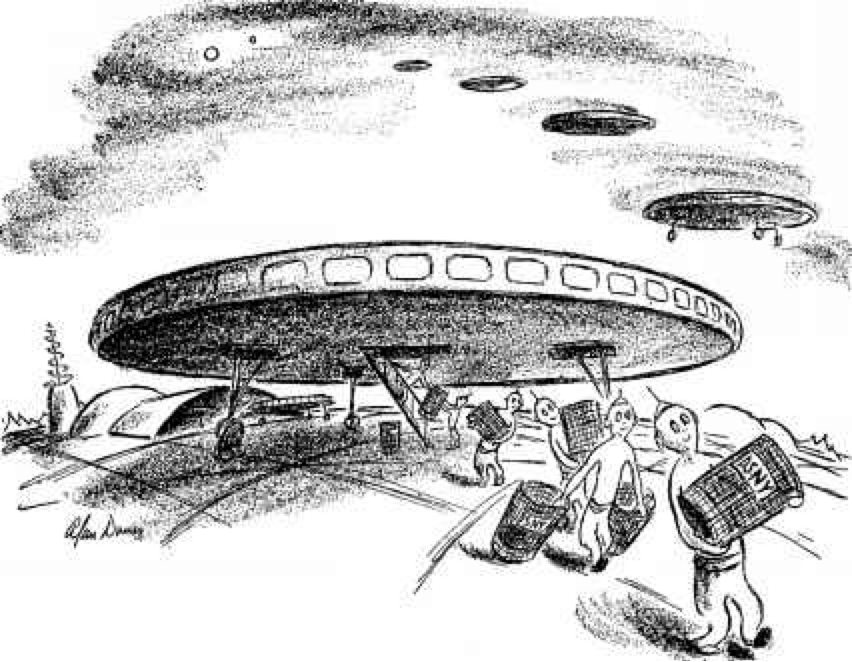
\includegraphics[scale=0.3]{aliens}
New Yorker cartoon by Alan Dunn in the New Yorker


 \column{0.5\textwidth}
%\begin{block}{}
In the Spring of 1950 the New York newspapers reported simultaneously the disappearance of public trash cans and numerous flying saucer observations. 
\vspace{0.5cm}

Fermi was at Los Alamos in the summer of 1950. One day, he was chatting to Edward Teller and Herbert York and Emil Konopinski told them of the Dunn cartoon. Fermi remarked wryly that Dunn's was a reasonable theory because it accounted for two distinct phenomena: the disappearance of trash cans and the reports of flying saucers. 
%\end{block}
\end{columns}
\end{frame}

%%%%%%%%%%%%%%%%
\begin{frame}
\frametitle{Where is everybody?}

\begin{columns}
\column{0.40\textwidth}
\includegraphics[scale=0.25]{aliensfermi.jpeg}

 \column{0.5\textwidth}
\begin{itemize}

\item During lunch Fermi asked suddenly: ``Where is everybody?'' His lunch partners immediately understood that he was talking about aliens. York recalls that Fermi made a series of rapid calculations and concluded that we should have been visited long ago and many times over.

\item Apparently Fermi didn’t saw the outcome of his calculation as a paradox. He also didn't doubt that extraterrestrial civilizations might exist, but supposed that interstellar travel wasn’t feasible or that alien had simply never found Earth in the vastness of the galaxy.    
\end{columns}
\end{frame}

%%%%%%%%%%%%%%%
\begin{frame}
\frametitle{The Drake equation}

\begin{columns}
\column{0.40\textwidth}
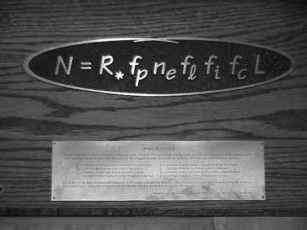
\includegraphics[scale=0.25]{drake}

 \column{0.5\textwidth}
\begin{itemize}

\item Represent the number of communicating Extraterrestrial Civilizations (ETCs) in the Galaxy by the symbol $N$. To estimate $N$ we multiply the following factors: the yearly rate $R$ at which stars form in the Galaxy; the fraction $f_p$ of stars that possess planets; the fraction $n_e$ of planets with environments suitable for life. The fraction $f_l$ of suitable planets on which life actually develops; the fraction of these planets on which life develops intelligence $f$; and the fraction $f_c$ of intelligent life-forms that develop a culture capable of interstellar communication. Finally, we need to know the time $L$, in years, that such a culture will devote to communication. Multiplying all these factors together results in the famous Drake's equation.

\item The Drake equation is a means of estimating the number of communicative ETCs in the Galaxy. Drake developed the equation so that it could form the agenda for the first ever SETI meeting (held at nrao Green Bank, WV, in 1961). The commemorative plaque is on the same wall that held the blackboard where the equation was first written.   
\end{columns}
\end{frame}
%%%%%%%%%%%%%%%%%

\begin{frame}
\frametitle{The Hart-Tipler argument}

\begin{columns}
\column{0.40\textwidth}
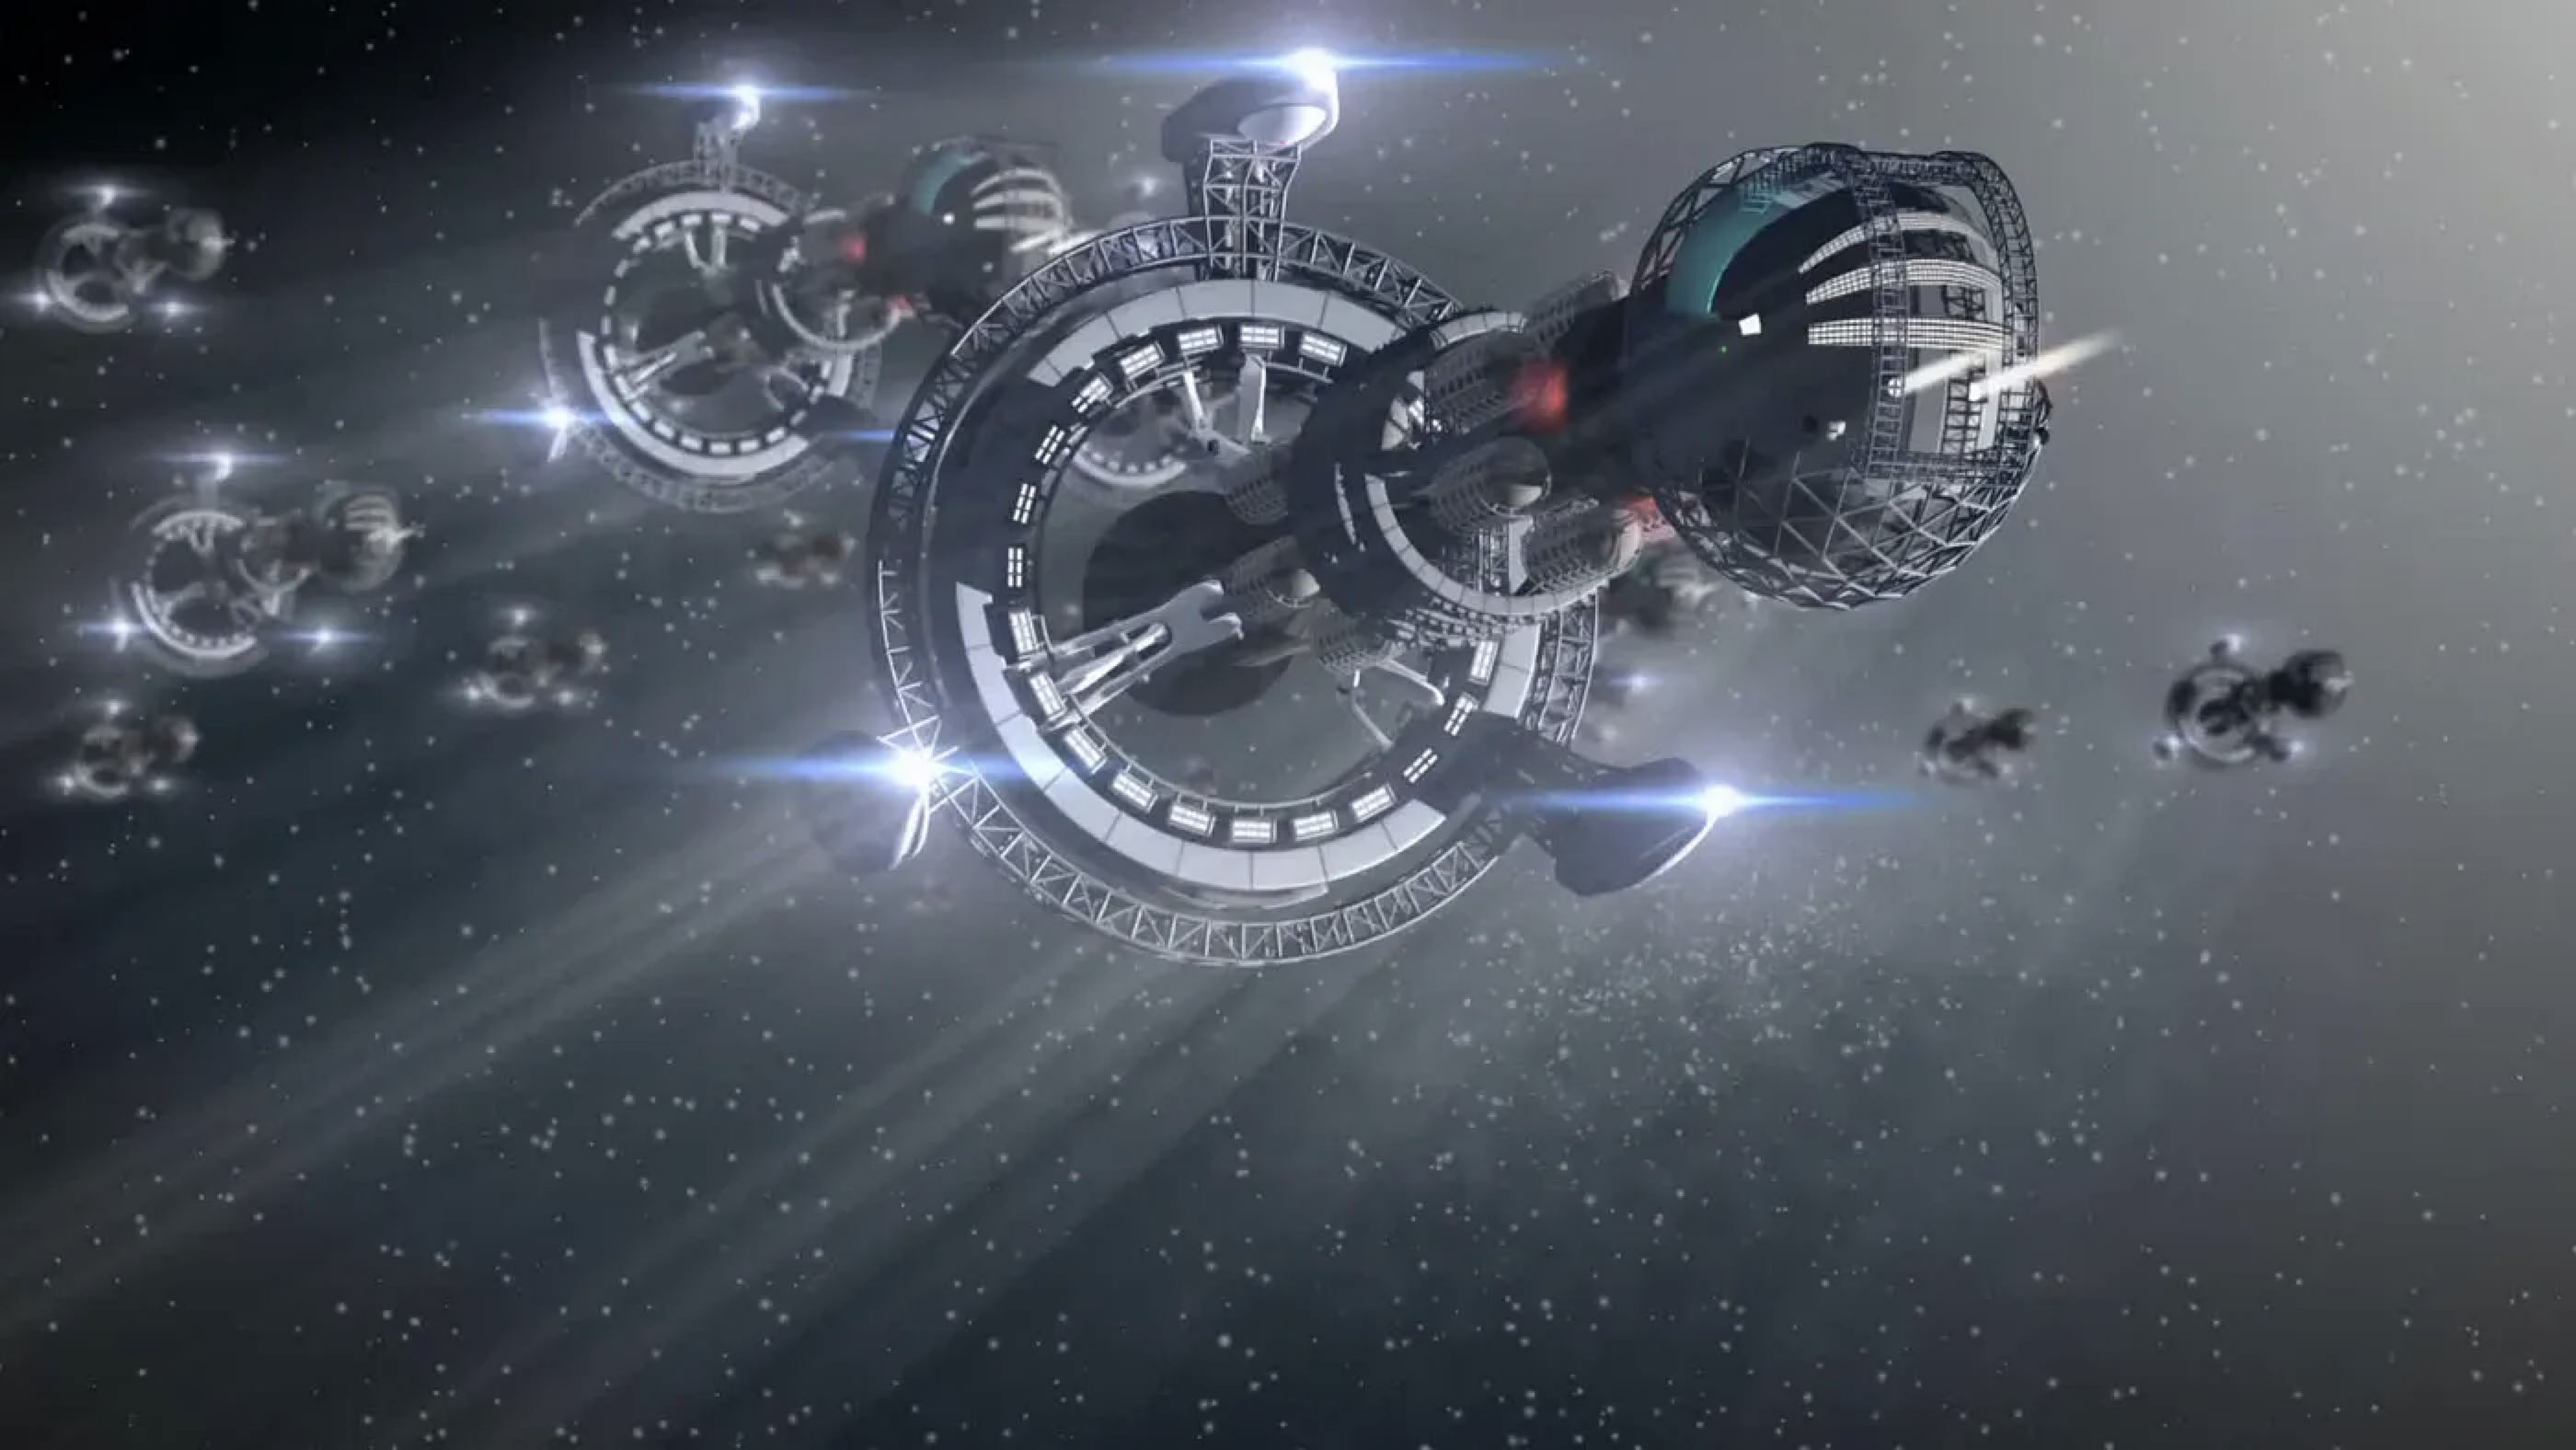
\includegraphics[scale=0.25]{spaceships}

Hart, Michael H. “Explanation for the Absence of Extraterrestrials on Earth.” Quarterly Journal of the Royal Astronomical Society, Vol. 16, 1975, pp.128–135.

“an extensive search for radio messages from other civilizations is probably a waste of time and money”


 \column{0.5\textwidth}
\begin{itemize}

\item In his 1975 paper, astronomer M. Hart speculated how long it would take hypothetical alien civilizations to colonize the Miky Way. He assumed that space-faring alien civilizations could proliferate with a colonization wavefront speed of 10 percent the speed of light (equal to the speed that colonization ships could spread throughout the galaxy). Given that the Milky Way is about 100 Myr across, colonization would take  about 1Myr, a tiny span of time compared with the age of the galaxy. 

\item Hart used this reasoning to argue for the nonexistence of advanced extraterrestrials in the Milky Way, since humans (latecomers in the history of the galaxy) have not found signs of their probes or colonization ships (nor any meaningful signal emitted by putative ``galactic centers''. Hart equated lack of observation to non-existence.  
\end{columns}
\end{frame}


%%%%%%%%%%%%%

\begin{frame}
\frametitle{The Neuman-Sagan  model}

\begin{columns}
\column{0.40\textwidth}
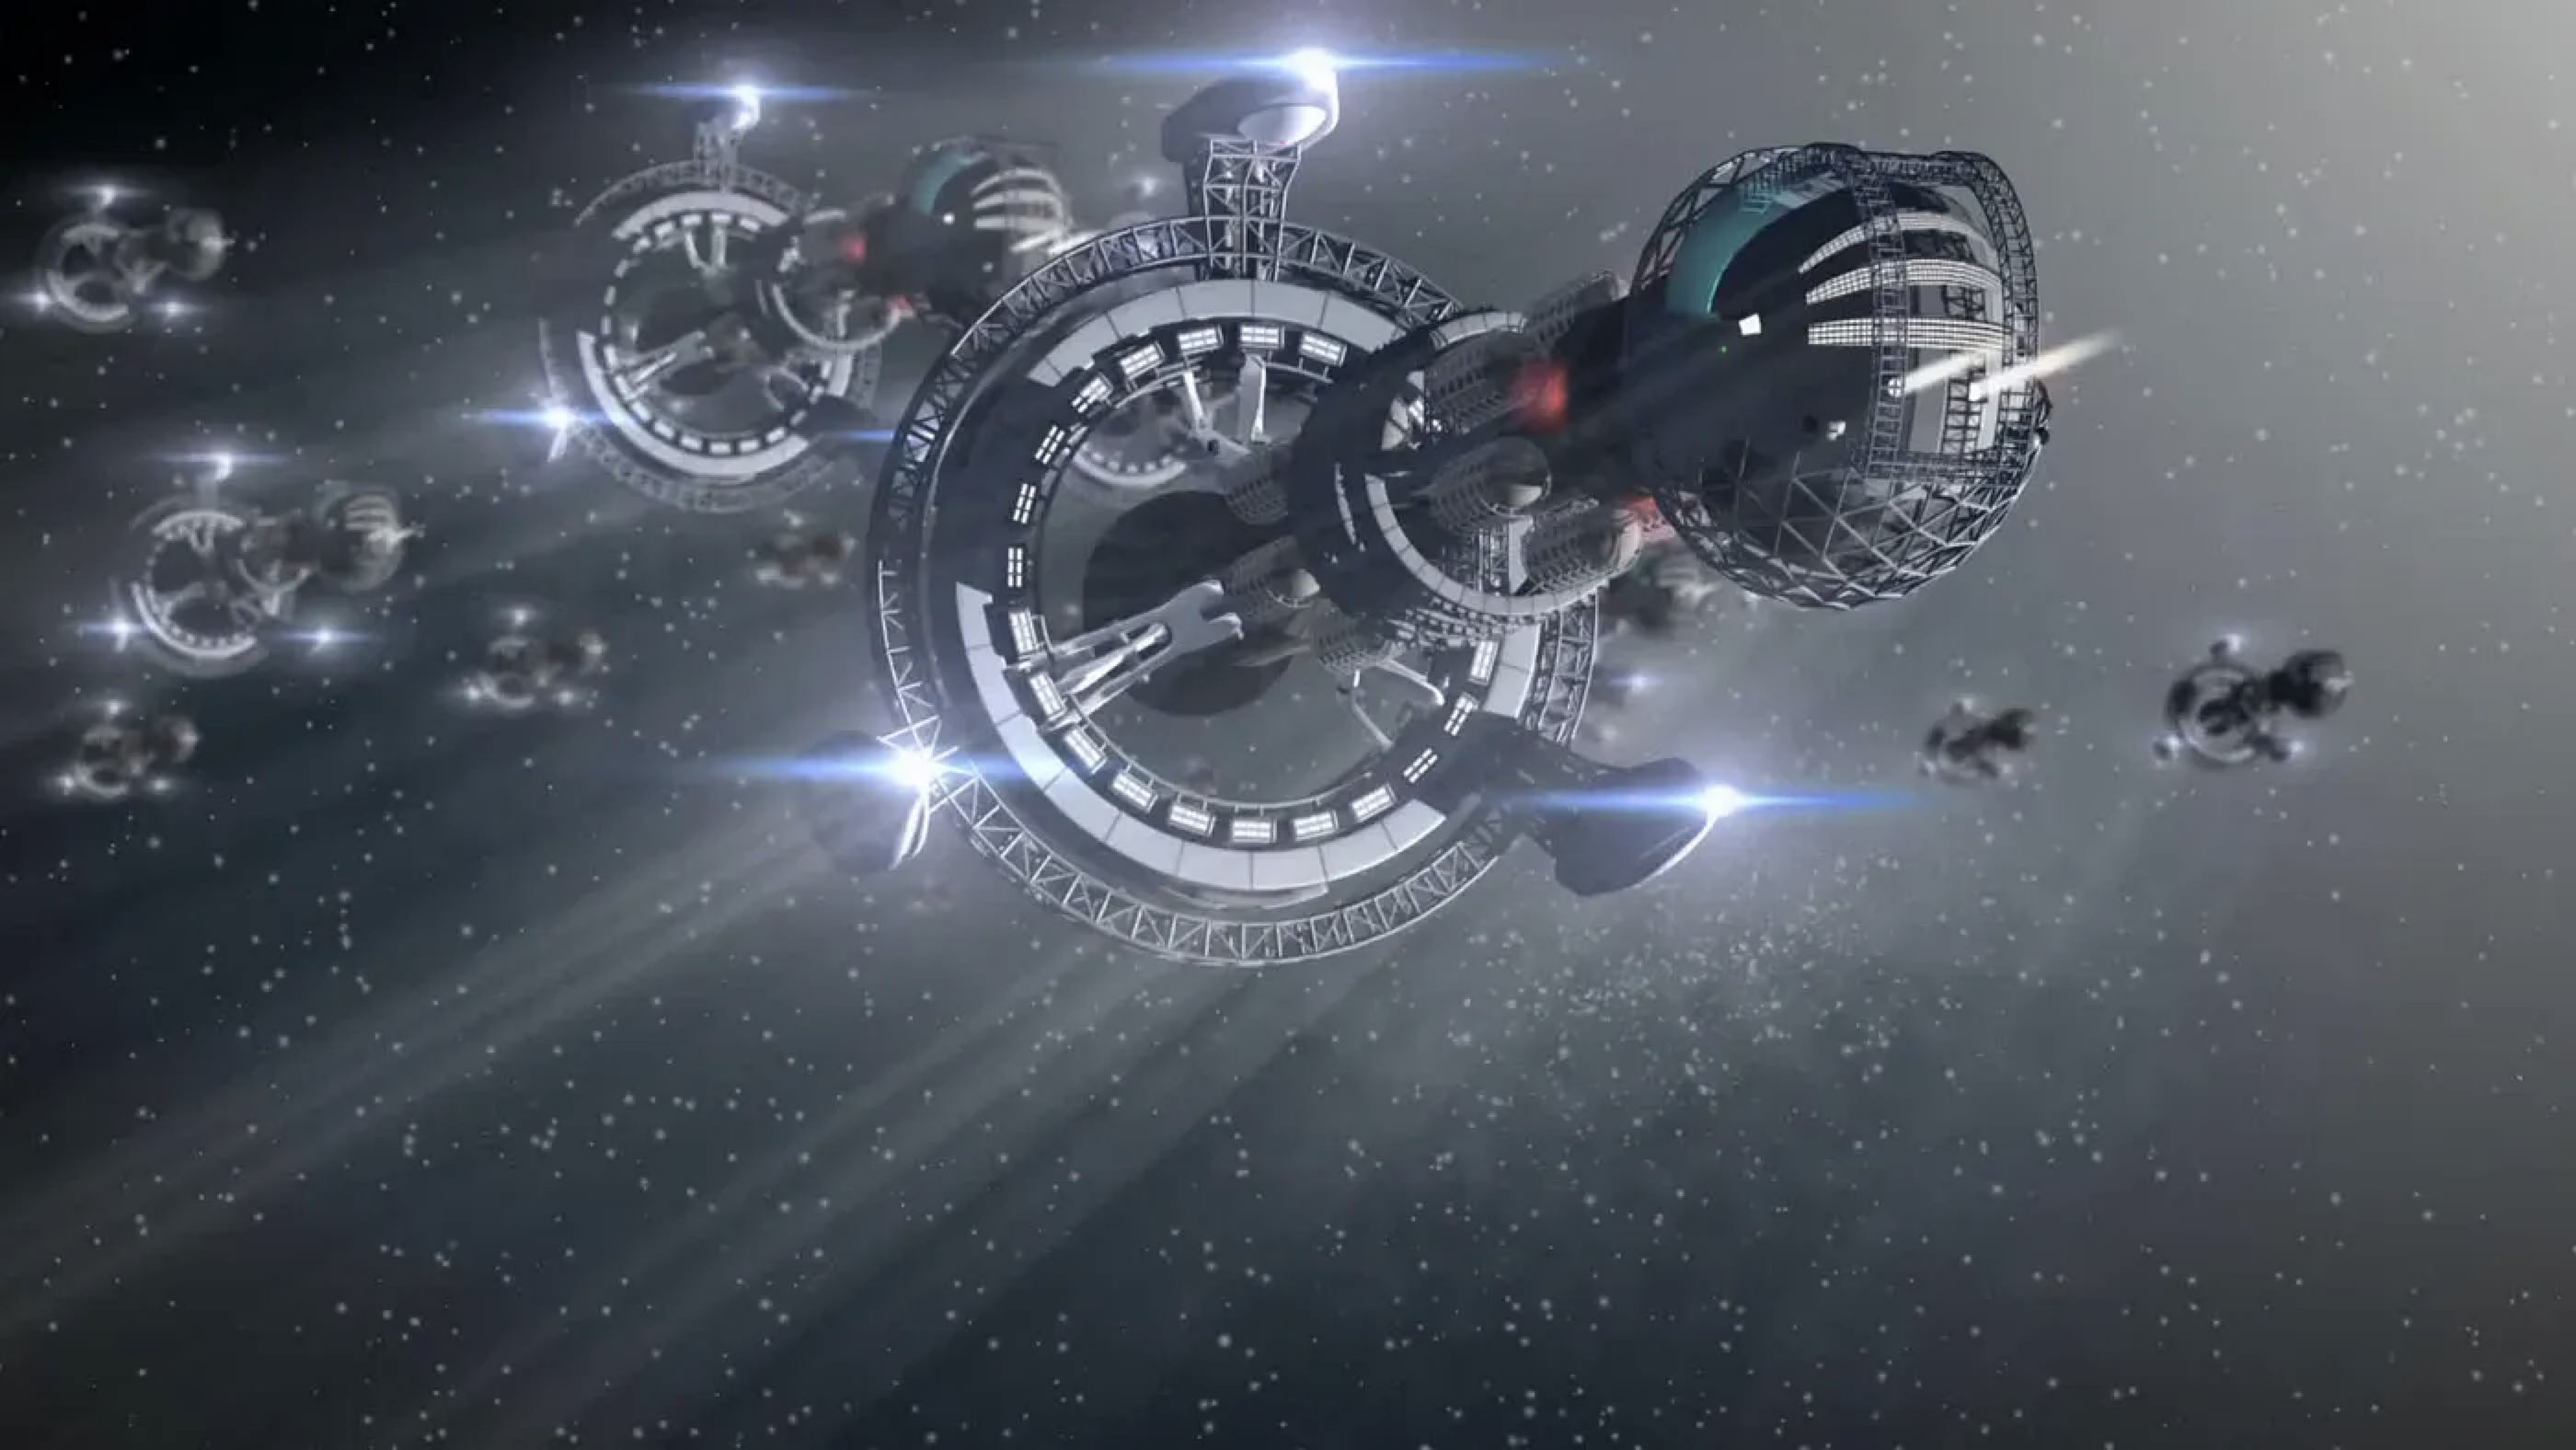
\includegraphics[scale=0.25]{spaceships}

Icarus, Volume 46, Issue 3, June 1981, Pages 293-327.

 \column{0.5\textwidth}
\begin{itemize}

\item In his 1975 paper, astronomer M. Hart speculated how long it would take hypothetical alien civilizations to colonize the Miky Way. He assumed that space-faring alien civilizations could proliferate with a colonization wavefront speed of 10 percent the speed of light (equal to the speed that colonization ships could spread throughout the galaxy). Given that the Milky Way is about 100 Myr across, colonization would take  about 1Myr, a tiny span of time compared with the age of the galaxy. 

\item Hart used this reasoning to argue for the nonexistence of advanced extraterrestrials in the Milky Way, since humans (latecomers in the history of the galaxy) have not found signs of their probes or colonization ships (nor any meaningful signal emitted by putative ``galactic centers''. Hart equated lack of observation to non-existence.  
\end{columns}
\end{frame}


%%%%%%%%%

%\begin{frame}
%%\frametitle{FP revisited}
%\begin{block}{}
%\center{\Huge FP Revisited}
%\end{block}
%\end{frame}

\begin{frame}
\frametitle{Formulations of the Fermi Paradox}
\begin{itemize}
\item {\bf ProtoFP}: The absence of extraterrestrials on Earth is incompatible with the multiplicity of extraterrestrial civilisations and our conventional assumptions about their capacities. 
\item {\bf WeakFP}: The absence of extraterrestrials or their artefacts on Earth and in the Solar System is incompatible with the multiplicity of extraterrestrial civilisations and our conventional assumptions about their capacities. ProtoFP and WearkFP are {\em weak} formulations of the FP, since, even in a Galaxy teeming with advanced civilisations, there are many ways to explain non-direct observations {\em on Earth or the solar system}.
\item {\bf StrongFP}: The lack of any intentional activities or manifestations or traces of extraterrestrial civilisations in our past light cone is incompatible with the multiplicity of extraterrestrial civilisations and our conventional assumptions about their capacities. This is much hard to explain, since it involves a much larger volume (thus many more potential civilisations) and tries to detect any signal arising from them. As an example, our primitive Earth civilisation has been signalling its presence of the last two hundred years or so. 
\end{itemize}

\end{frame}

%\begin{frame}
%\frametitle{More paradoxical than ever}
%
%\begin{columns}
%\column{0.35\textwidth}
%\includegraphics[scale=0.03]{earthlike.jpeg}
%
%The number of Sun-like stars that could have an Earth-like planet in the habitable zone may be as high as  22\%. 
%
%%(https://www.pnas.org/doi/full/10.1073/pnas.1319909110)
%
%
% \column{0.5\textwidth}
%%\begin{block}{}
%
%A number of recent discoveries make the problem objectively more disturbing than ever.
%
%\vspace{0.5cm}
%
%For example: in 1950 one could argue that planetary solar systems were rare (or even unique), or that ``Goldilocks'' conditions happened exceptionally or  that Earth is in the extreme early tail of the planet-age distribution, being among the oldest, if not the oldest habitable planet in the Milky Way. Those hypothesis, not unreasonable at the time would have ``solved'' the paradox, leading to Earth being the first civilisation in the Galaxy. 
%\end{columns}
%\end{frame}
%
%\begin{frame}
%\frametitle{Recent scientific advances suggest we are not singular}
%\begin{itemize}
%\item Confirmation of the rapid origination of life
%on early Earth (Mojzsis et al. 1996) offers a strong probabilistic
%support to the idea of many planets in the
%Milky Way inhabited by at least the simplest
%lifeforms (Lineweaver and Davis 2002).
%\item Discovery of extremophiles and the general resistance of simple lifeforms to much more severe environmental stresses than it had been
%thought possible earlier (Cavicchioli 2002) suggests that the number and
%variety of cosmic habitats for life are probably
%much larger than conventionally imagined.
%\item Improved understanding in molecular biology and biochemistry leading to heightened
%confidence in the theories of naturalistic origin
%of life or {\em abiogenesis} (Lahav et al. 2001, Ehrenfreund et al. 2002, Bada 2004). 
%\item Improved understanding of the origin of intelligence and technological civilization
%({\em noogenesis}) also supports naturalistic origin (e.g. Chernavskii 2000).
%\end{itemize}
%
%\begin{block}{}
%In short, recent scientific advances suggest that life and (to a lesser degree) intelligence should be common in the Universe. 
%\end{block}
%\end{frame}
%
%\begin{frame}
%\frametitle{Technological advances suggest that Galaxy colonisation is possible}
%\begin{itemize}
%\item Exponential growth of the technological civilization on Earth (e.g., technological waves of which IAG is the last, see Suleiman 2023) suggests that civilisations
% experience exponential technological grow. 
%\item An outstanding question is whether energy will limit technological development on Earth. The optimistic view is that it will not. Technological civilisations can harness eventually nuclear fusion as well as (all) the energy provided by their star. 
%\item Interstellar travel appears more feasible in both the classical sense
%(e.g. Andrews 2003), and in the more efficient
%form of sending interstellar probes.
%%\item Theoretical grounding for various astroengi-
%%neering/macroengineering projects (Badescu
%%1995, Badescu and Cathcart 2000, 2006, Ko-
%%rycansky et al. 2001, McInnes 2002) potentially detectable over interstellar distances.
%%Especially important in this respect is the
%%possible combination of astroengineering and
%%computation projects of advanced civiliza-
%%tions, like those envisaged by Sandberg (1999).
%\item We have observed many galaxies, and not a single civilization of Kardashev's Type III has been
%found, in spite of the huge volume of space
%surveyed (Annis 1999b).
%\end{itemize}
%
%\begin{block}{}
%StrongFP is a more paradoxical than ever.  
%\end{block}
%\end{frame}

\begin{frame}
\frametitle{Kardashev Classification}

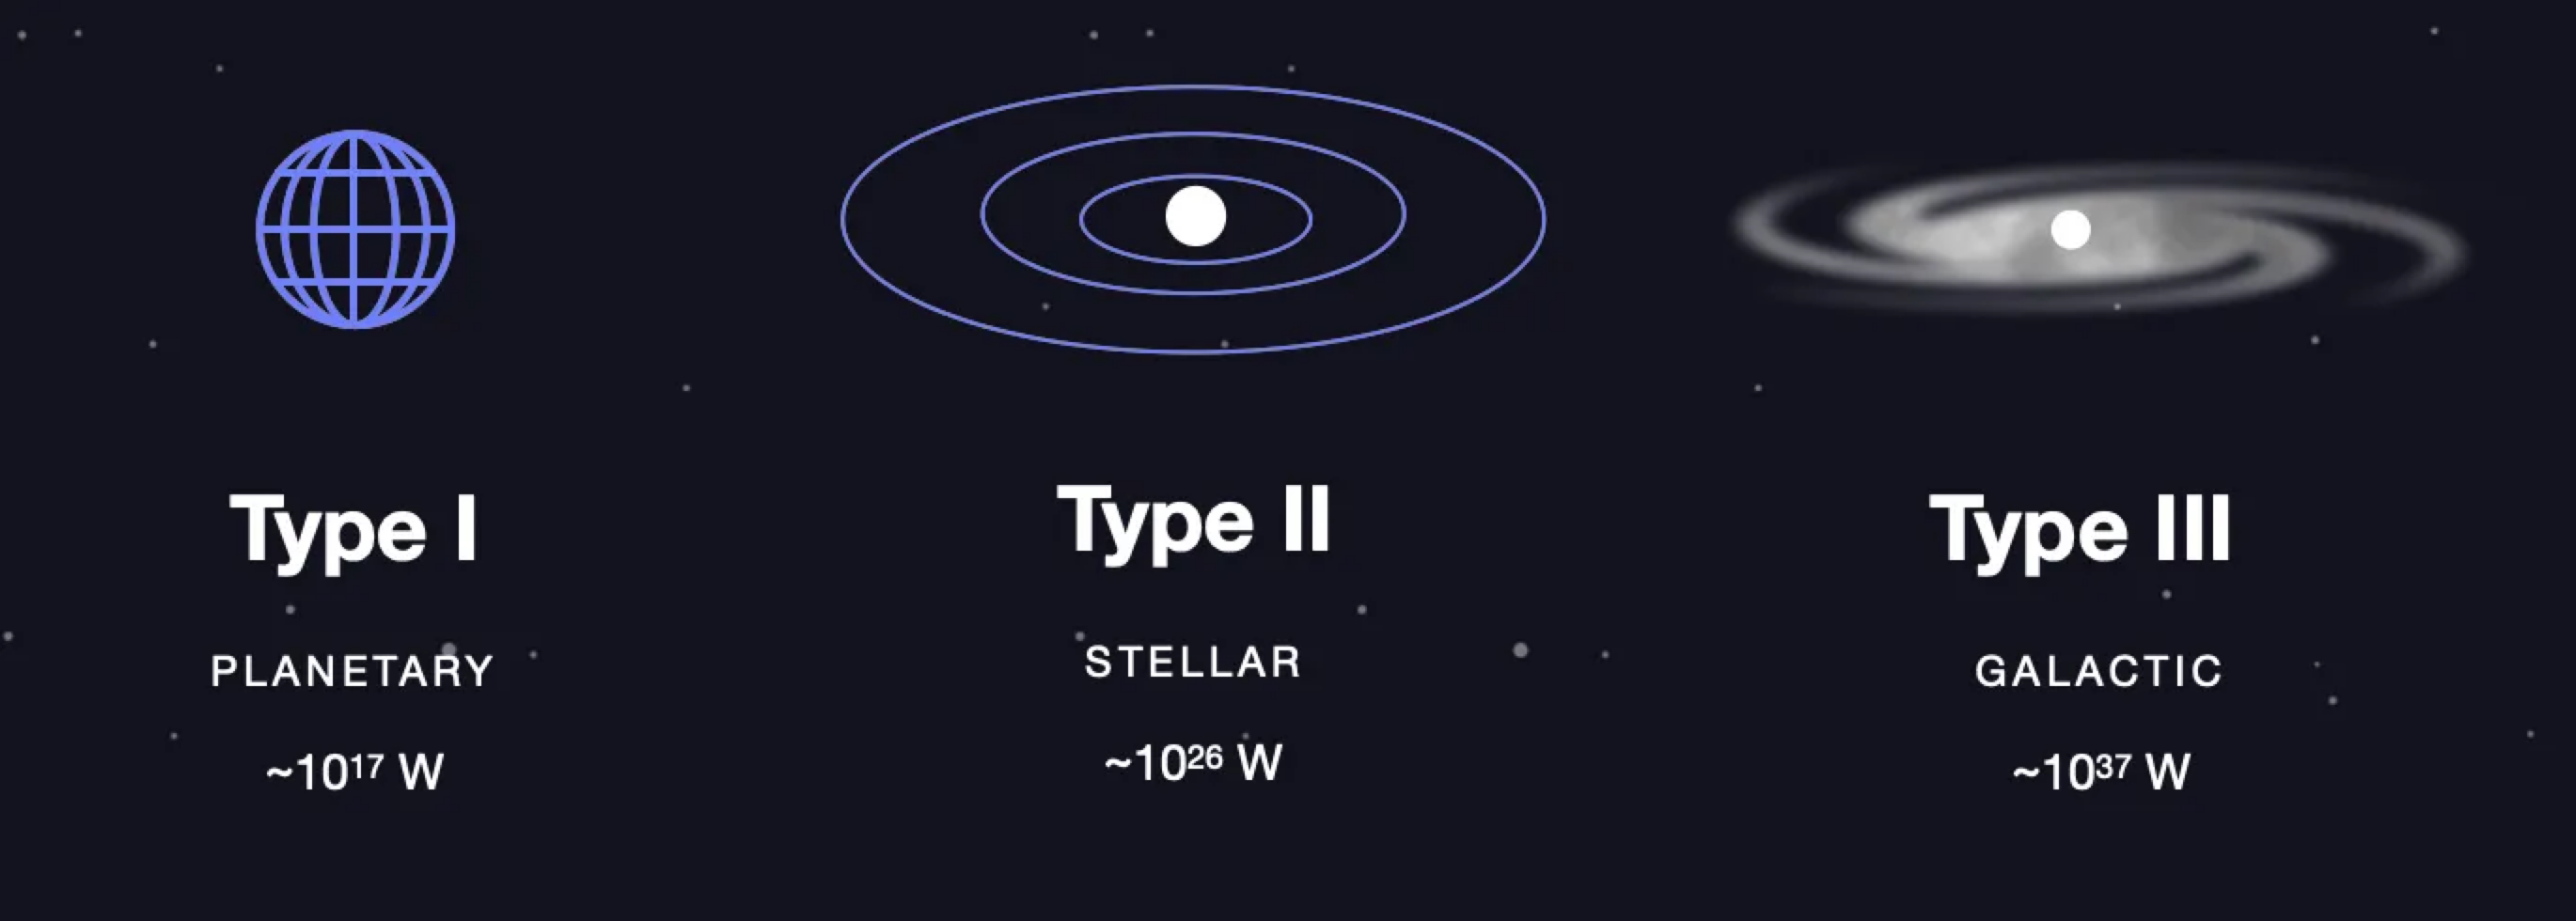
\includegraphics[scale=0.15]{kardashev.png}

The Kardashev scale (1964) ranks the technological capabilities of a civilization based on its ability to manipulate and exploit energy. 
\begin{itemize}
\item {\bf Type 0} uses energy sources like coal, oil, and natural gas.
\item {\bf Type I} has complete control over the energy of its host planet.
\item {\bf Type II} can harness the power of its sun and control the entire solar system.
\item {\bf Type III} spans the entire galaxy, colonizing and controlling numerous systems. 
\end{itemize}

Humanity is considered a type 0 civilization (0.72 according to Carl Sagan). It is estimated that we will reach type I in 100–200 years, type II in $\sim$ 10 kyrs, and type III in $10^5--10^6$ to kyrs.

\end{frame}

\begin{frame}
\frametitle{Fermi-Hart timescale}

\begin{columns}
\column{0.5\textwidth}
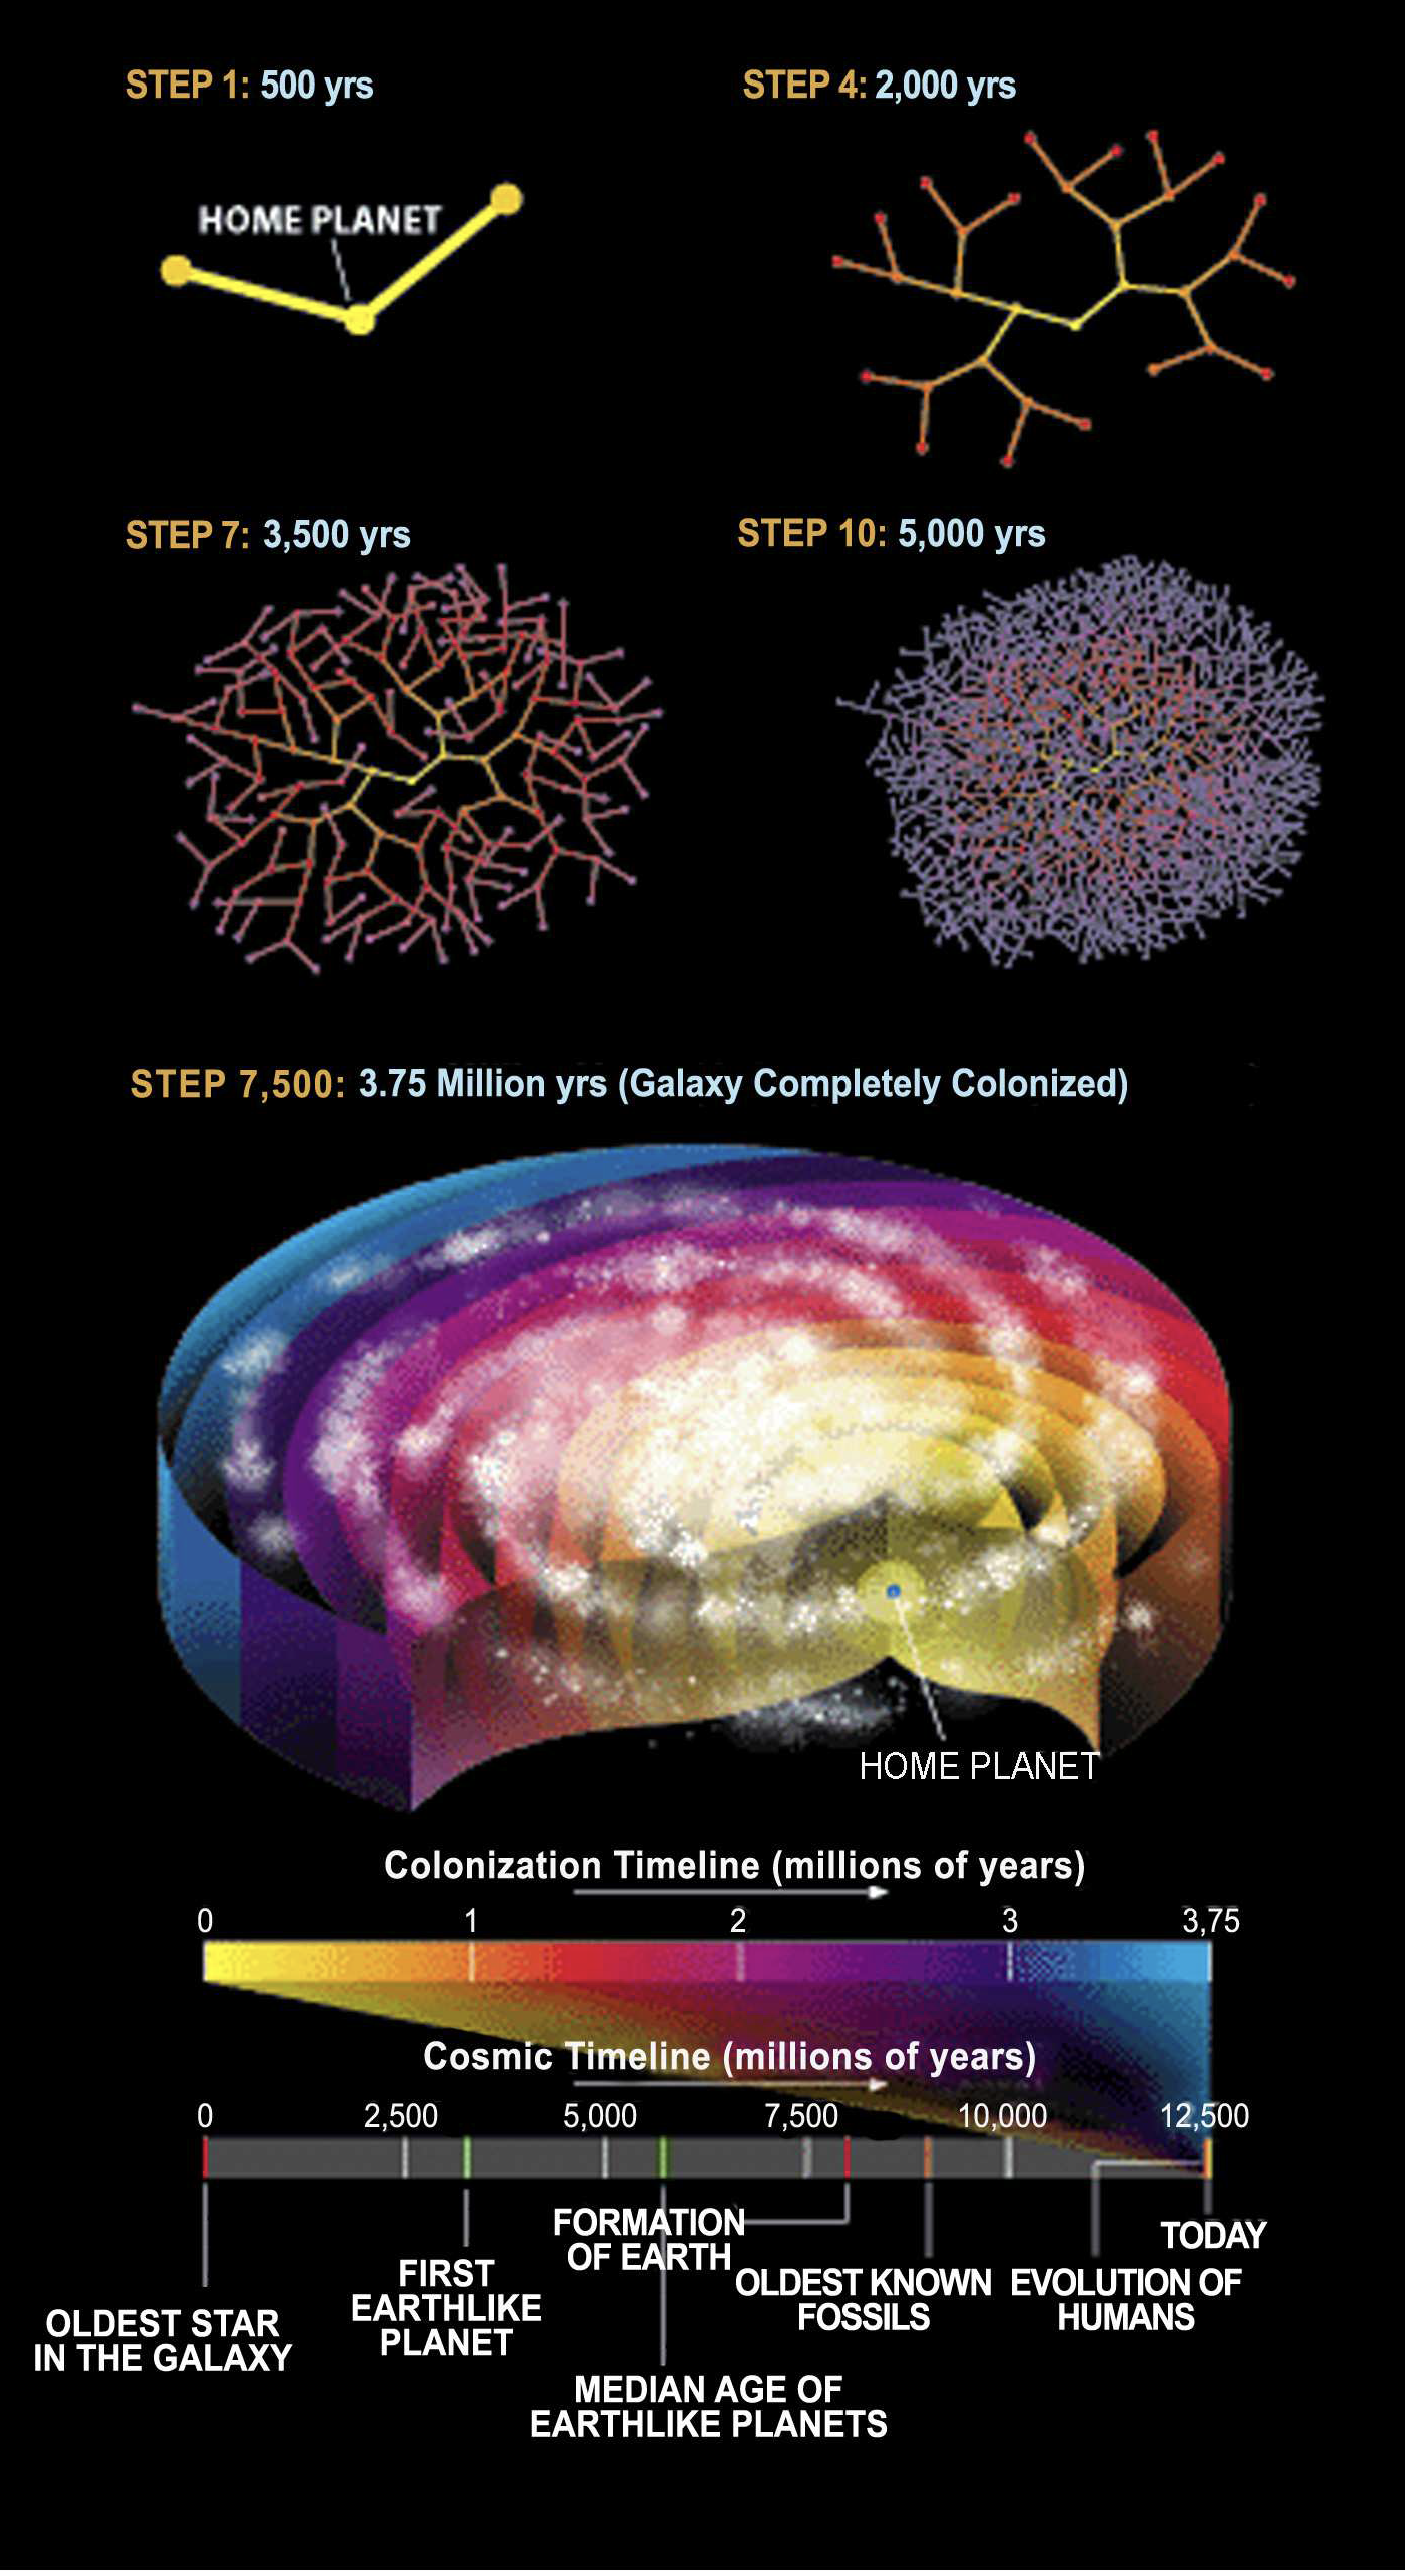
\includegraphics[scale=0.5]{colonisation.png} 

 \column{0.4\textwidth}
Fermi’s paradox in a model with slow von Neumann probes, giving a typically low Fermi-Hart timescale for the colonization of the Milky Way. The relevant timescales are also shown.

$t_{FH} \sim 10^6-10^8$ yr
\end{columns}
\end{frame}
\begin{frame}
\frametitle{The Galaxy-Solar system timescale}

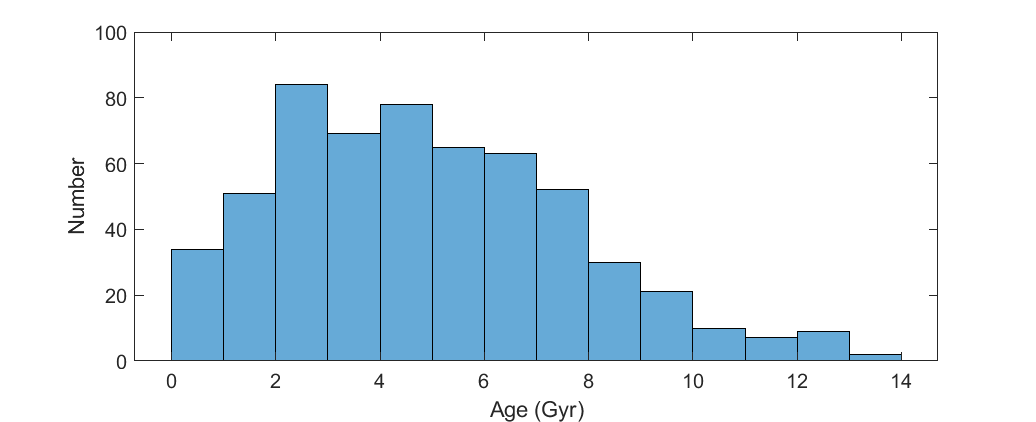
\includegraphics[scale=0.45]{M00s9.png}


The formation of Earth-like planets started likely more than 9 Gyr ago. The median age of planes in the galaxy is $t_M =6.4 \pm 0.9$ Gyr, while the solar system (and Earth) have an age $t_E =4.5681 \pm 0.004$ Gyr. This means that planet formation in the galaxy reached its peak  $t_M - t_E = 1.9 \pm 0.9$ Gyr before our planet completed its original accretion. Also, consider that the older planes formed $\sim$ 4 Gyr before Earth.  

\end{frame}

\begin{frame}
\frametitle{The FP reformulated}

\begin{block}{}

$$ t_{FH} <<< t_M - t_E$$

\end{block}

\vspace{0.5cm}
\begin{itemize}
\item
Most of the habitable sites in the Milky Way (and most likely elsewhere) are billions of years older than Earth, giving ample time for KTIII civilisations to form. Thus, the Galaxy should be already colonized and/or, evidence for KTIII civilisations in other galaxies should be observable. 
%
%\vspace{0.5cm}
\item
Even more generally, we need not consider the direct physical contact between an extraterrestrial civilization and Earth or the Solar System. It is sufficient to consider a weaker requirement: namely that no extraterrestrial civilizations are detectable by any means from Earth at present. In particle physics parlance we could ask why the ``contact cross-section'' in the Milky Way at present is so small in comparison to naive expectations.
\end{itemize}
%{\em provided that we accept the straightforward Copernican assumption}.
%\end{columns}
%\end{frame}
\end{frame}

\begin{frame}
\frametitle{The Philosophy department's nightmare.}

{\em Hi guys, we are physicist and we are here to help!}
\vspace{0.5cm}

Disclaimers: 

\begin{itemize}
\item In this talk I am going to use profusely terms  such as``intuitive'', ``accepted'', ``common sense'', ``practical'', or ``effective''.  If you feel that I am trying to avoid rigorous definitions, talk to my lawyer.  
\item Since I am not providing a rigorous definition of ``intelligence''  (or, God forbids, ``conscience''), then I don't need to be precise when referring to ``extraterrestrial intelligence''. Extraterrestrial intelligent beings are taken as entities which are able to communicate with. 
\item I will stick to a few philosophical concepts as ``desirable guides'' to understand FP. Specifically, I will invoke Realism, Naturalism, Copernicanism, Gradualism (this one tongue-in-cheek) and Hardness as guidelines to  ``grade'' potential explanations of the FP. In my definitions of the above ``ism's'' I will also be ``intuitive'', and my ``grading'' may be totally biased. Again, my lawyer will be happy to discuss any pertinent legal issues with those of you who rather chase me out of the room.  
\end{itemize}

\end{frame}

%\begin{frame}
%\frametitle{Key concepts related with Fermi Paradox}
%
%\begin{columns}
%\column{0.35\textwidth}
%\includegraphics[scale=0.06]{impossible.jpeg}
%
%Fermi Paradox may sits well into a famous class of mathematical problems popularised by Martin Gardner and often known as "impossible puzzles",
%
%
% \column{0.5\textwidth}
%%\begin{block}{}
%Scientific and technological: Intelligence, civilisation, technology, evolution, interstellar travel, detectability. Philosophical:  Realism, Copernican assumption, naturalism,  to name a few. 
%
%\vspace{0.5cm}
%
%The Paradox sits well into a famous class of mathematical problems popularised by Martin Gardner and often known as "impossible puzzles", where players have insufficient information to produce a solution, but gain additional knowledge from the fact that the other players cannot solve it either.
%
%%\end{block}
%\end{columns}
%\end{frame}



%\begin{frame}
%\frametitle{Detectability \& synchronisation}
%
%\begin{itemize}
%\item {\bf Detectability} of an intelligent species is a metric quantifying the difficulty to detect the presence of such a species from interstellar distances. The {\em soft} detectability condition would apply to detectability within the Galaxy, thus a range from less than a parsec to several thousand parsecs. The {\em hard} condition would extend detectability to species in the past light cone (e.g., the set of accesible galaxies from our view point). 
%\item {\bf Synchronisation}  implies that other intelligent species are contemporary to us, a concept way more restrictive than detectability. 
%\end{itemize}

%\end{frame}

\begin{frame}
\frametitle{Philosophical handles: Realism}

\begin{itemize}
\item {\bf Scientific, ``naive'' or ``common sense'' realism}.  Working philosophy of most of science (as well as everyday life), implying that there is a material world out there, composed of objects that occupy space, have a duration in time, and have properties such as size, mass, shape, texture, smell, taste, and colour. These properties are usually perceived correctly and obey the laws of physics. 
\item {\bf Realism applied to FP} states that there are no traces of extraterrestrial intelligent presence (ETI) detected either directly or indirectly.

\item {\bf Realism is a methodological assumption} used in scientific research. Neither me, nor my lawyer will consider as valid solutions of FP that violate the Realism requirement (e.g., UFO = ETI theories).  
\end{itemize}

\end{frame}

\begin{frame}
\frametitle{Philosophical handles: Naturalism}

{\em Monsiuer, Je n'avais pas besoin the cette hypotehèse (Laplace to the First Consul of French Republic). }

\vspace{0.5 cm}
\begin{itemize}
\item A prohibition against invoking supernatural agents or events in scientific explanations.
\item Naturalism (at least on its soft version, which is good enough for this discussion) does not make hypothesis concerning the existence of supernatural agents, it just states that our explanatory mechanism should not invoke them either explicitly or implicitly.
\item Indeed, supernaturalism could solve easily the FP by postulating a unique divine creation in the Universe, as in Western monotheistic religions (although one could need to explain why the waste of resources, e.g, $10^{22}$ stars for a single inhabited planet). 
\end{itemize}
\end{frame}


\begin{frame}
\frametitle{Naturalism and Abiogenesis}

\begin{itemize}
\item A necessary (naturalist) ingredient in any scientific account of life is the so-called {\bf continuity thesis}, that is the assumption that there is no unbridgeable gap between inorganic matter and living systems.
\item On the other hand, the question of how probable is the emergence of life has not been fully quantified. While the prevalent scientific view is that given the
 right physical conditions the emergence of life is highly probable, this is not a demonstrated fact, since we do not have yet a full description of the mechanisms that led to life from inorganic matter, nor have we been able to ``replicate'' life in the lab. 
\item An scenario in which the emergence of life turned out to be extremely improbable, could act as an ``early filter'' that would solve the FP, providing an explanation which would be ``de facto'' identical to the supernatural ``divine creation'' hypothesis mentioned above, while still respecting naturalism (extremely improbable does not mean impossible).  
\end{itemize}
\end{frame}

\begin{frame}
\frametitle{Naturalism and Noogenesis}

\begin{itemize}
\item The continuity thesis should also apply to the emergence of ``intelligence'' and ``conscience''. The situation here is more complex, since it is difficult to define what intelligence (or conscience) means.
\item On the other hand one could argue that intelligence (and conscience) are common phenomena on Earth. Examples of intelligent species include dolphins, whales and the great apes. We know of at least an intelligent Homo species (Neanderthals) not equivalent to Sapiens. Thus one could expect that the emergence of intelligence, once complex life evolves is highly probable.  
\item In 2023 is specially relevant to consider also post-biological intelligence, e.g, the emergence of (imminent?)  artificial intelligence.  Notice that many of the technical difficulties associated with interstellar travel (and thus to the expansion of advanced civilizations) only apply to biological, not post-biological (``machines'') beings, which could be the predominant form of intelligence in the Galaxy. 
\end{itemize}
\end{frame}

\begin{frame}
\frametitle{Philosophical handles: Copernicanism}
\begin{itemize}
\item {\bf Also called Principle of Typicality}. There is nothing special about Earth, the Solar System, or our Galaxy within large sets of similar objects throughout the universe (Sagan, Drake and others). In a somewhat broader sense, it indicates that there is nothing special about us as observers: our temporal or spatial location, or our location in other abstract spaces of physical parameters, chemical parameters, biological parameters, and so on, are typical or close to typical. 
\item Notice that, unlike Realism and Naturalism, Copernicanism is not a scientific must, although it has been a cornerstone of the scientific revolution and the ``great demotions'' that took Earth (and man) out of the center of the Universe. And yet, nothing prevents our planet, {\em a priory} from being an outlier in one or more aspects. As we will see soon, a full family of proposed solutions to the FP, grouped under the label of ``Rare Earth Hypothesis'' argue precisely so. 
\end{itemize}

\end{frame}

\begin{frame}
\frametitle{Philosophical handles: Non-exclusivity}
\begin{itemize}
\item {\bf Also called Principle of Hardness}.  Favours those hypotheses which involve a smaller number of local causes. 
\item For example, the FP  is not resolved by postulating that the Galaxy contained only one  single old civilisation (apart of us), which self-destructed itself in a nuclear holocaust (why just one?). Instead we would need to postulate that all civilizations self-destruct soon after developing nuclear weapons. This, in turn, requires many local causes acting independently in a uniform way to achieve the desired explanatory end. In other words, such solution is exclusive (or ``soft''). In contrast, a non-exclusive (or ``hard'') solution rely on a small number of independent causes. For instance, the hypothesis that a GRB can cause mass extinction over a large portion of the Galaxy and thus arrest evolution towards advanced technological society is a hard solution. 
\end{itemize}

\end{frame}

\begin{frame}
\frametitle{Philosophical handles: Gradualism and Catastrophism}
\begin{itemize}
\item This is the notion that changes at planetary (and Galactic level) have occurred in a gradual (rather than catastrophe-driven) way. 
\item As I will discuss later this principle appears weaker than all those discussed above and in fact one could argue that the existence of great mass extinctions on Earth some of them clearly provoked by catastrophes (such as the meteorite that killed the dinosaurs 65 Myr ago) prove that ``naive gradualism'' doesn't hold water. 
\item An alternative view is that of ``punctuated gradualism'', e.g, periods of smooth, gradual evolution punctuated by rare catastrophes. This view is often referred to as neo-catastrophism. 
\end{itemize}

\end{frame}

\begin{frame}
\frametitle{Classification of FP solutions}

\begin{itemize}
\item Proposed by Cirkovic in 2009\footnote{Serb. Astron. J. } 178 (2009), 1 - 20}.
\end{{itemize}
\includegraphics[scale=0.75]{FPclassification.pdf}

\end{frame}

\begin{frame}
\frametitle{Solipsist Soluitions}

Solipsist solutions propose that extraterrestrials are or have been present in our vicinity, but have so far been undetected. 
%The reasons for such non detectability are varied and span a large family of hypothesis. Among them:

\begin{enumerate}
\item {\bf UFO's} have been observed and are of extraterestial origin. 
\item {\bf The Zoo hypothesis} of Ball (1973) and the related {\bf Interdict hypothesis} of Fogg (1987), suggest that there is a uniform cultural policy of advanced extraterrestrial civilizations to avoid any form of contact (including having a visible manifestations) with the newcomers to the ``Galactic Club''.
\item {\bf Directed panspermia} of Crick and Orgel (1973) suggests that Earth has indeed been visited in a distant past with very obvious consequences ---namely the existence of life on Earth! 
\item {\bf The Planetarium hypothesis} of Baxter (2000) suggests that our astronomical observations do not represent reality, but a form of illusion, created by an advanced technological civilization capable of manipulating matter and energy on interstellar or Galactic scales.
\item {\bf The Simulation hypothesis} of Bostrom (2003), suggest that we live in a computer simulation of an advanced technological civilization inhabiting the ``real'' universe.
\end{enumerate}

\end{frame}

\begin{frame}
\frametitle{Difficulties with the Solipsist Solutions}
\begin{itemize}
\item Most of the SS are either untestable ---like the eponymous metaphysical doctrine---, or testable only in limit of very long temporal and spatial scales. In other words, they violate one of our basic guidelines which I have referred to as  ``naive'' or ``practical'' scientific realism.

\item Many of them, but not all, violate the non-exclusivity (hardness) principle. This is, for instance, obvious in Zoo, Interdict or Planetarium scenarios, since they presume a large-scale cultural uniformity.

\item Directed panspermia has some additional problems – notably the absence of any further manifestations of our ``parent civilization'', in spite of its immense age. The hypothesis appears quite similar to the metaphysical notion of a God that creates the Universe and then, ``goes in vacation'', remaining invisible thereafter. Yes ``accidental'' panspermia may be about to happen in the Solar System, one our species expands to Mars and beyond. 
\end{itemize}
\end{frame}

\begin{frame}
\frametitle{Rare Earth Solutions}
The Rare Earth hypothesis (REH, Ward \& Donal, 2000) claims that, while simple microbial life is probably ubiquitous throughout the Galaxy, complex biospheres, like the terrestrial one, are very rare due to the exceptional combination of many distinct requirements:
\begin{itemize}
\item {\bf Circumstellar habitable zone}: a habitable planet needs to be in the very narrow interval of distances from the parent star.
\item {\bf Rare Moon}: having a large moon to stabilize the planetary axis is crucial for the long- term climate stability.
\item {\bf Rare Jupiter}: having a giant planet (``Jupiter'') at right distance to deflect much of the incoming cometary and asteroidal material enables sufficiently low level of impact catastrophes.
\item {\bf Rare elements}: Radioactive elements (especially U and Th) need to be present in the planetary interior in sufficient amount to enable plate tectonics and functioning of the carbon-silicate cycle.
\item {\bf Rare magnetosphere}, essential to deflect cosmic rays.  
\end{itemize}
\end{frame}


\begin{frame}
\frametitle{REH and the complexity of life (and intelligence)}

\begin{itemize}
\item {\bf Rare ``evolutionary pumps"} such as massive glaciations and bolide impacts.
\item {\bf Rare Cambrian-explosion analogs}, meaning the diverse and low-probability factors may have led to the emergence of eukaryotic cells, sexual reproduction, and the Cambrian explosion of animal, plant, and fungi phyla.  
\item {\bf Rare humans}. The evolution of human beings and of human intelligence may have required yet further specific events and circumstances, all of which are extremely unlikely to have happened were it not for the Cretaceous--Paleogene extinction event 66 million years ago removing dinosaurs as the dominant terrestrial vertebrates. 
\end{itemize}


\end{frame}

\begin{frame}
\frametitle{Plausibility of REH}
\begin{itemize}
\item It shows that the emergence of life (and then complex intelligence) on a planet requires the confluence of many factors, each one highly improbable. If the product of all those factors yield a number sufficiently small, then the space-temporal distribution of civilisations must be rarified enough as to explain the FP (e.g, intelligent species may be separated by many thousands of light-years and sparsely distributed on time). In other words, REH offers a rationale to explain why our civilisation on Earth may be unique or ``unique in practice'' in the Galaxy (while still conceding that life may be common). 
\end{itemize}
\end{frame}

\begin{frame}
\frametitle{REH and the GHZ}
\begin{columns}
\column{0.55\textwidth}

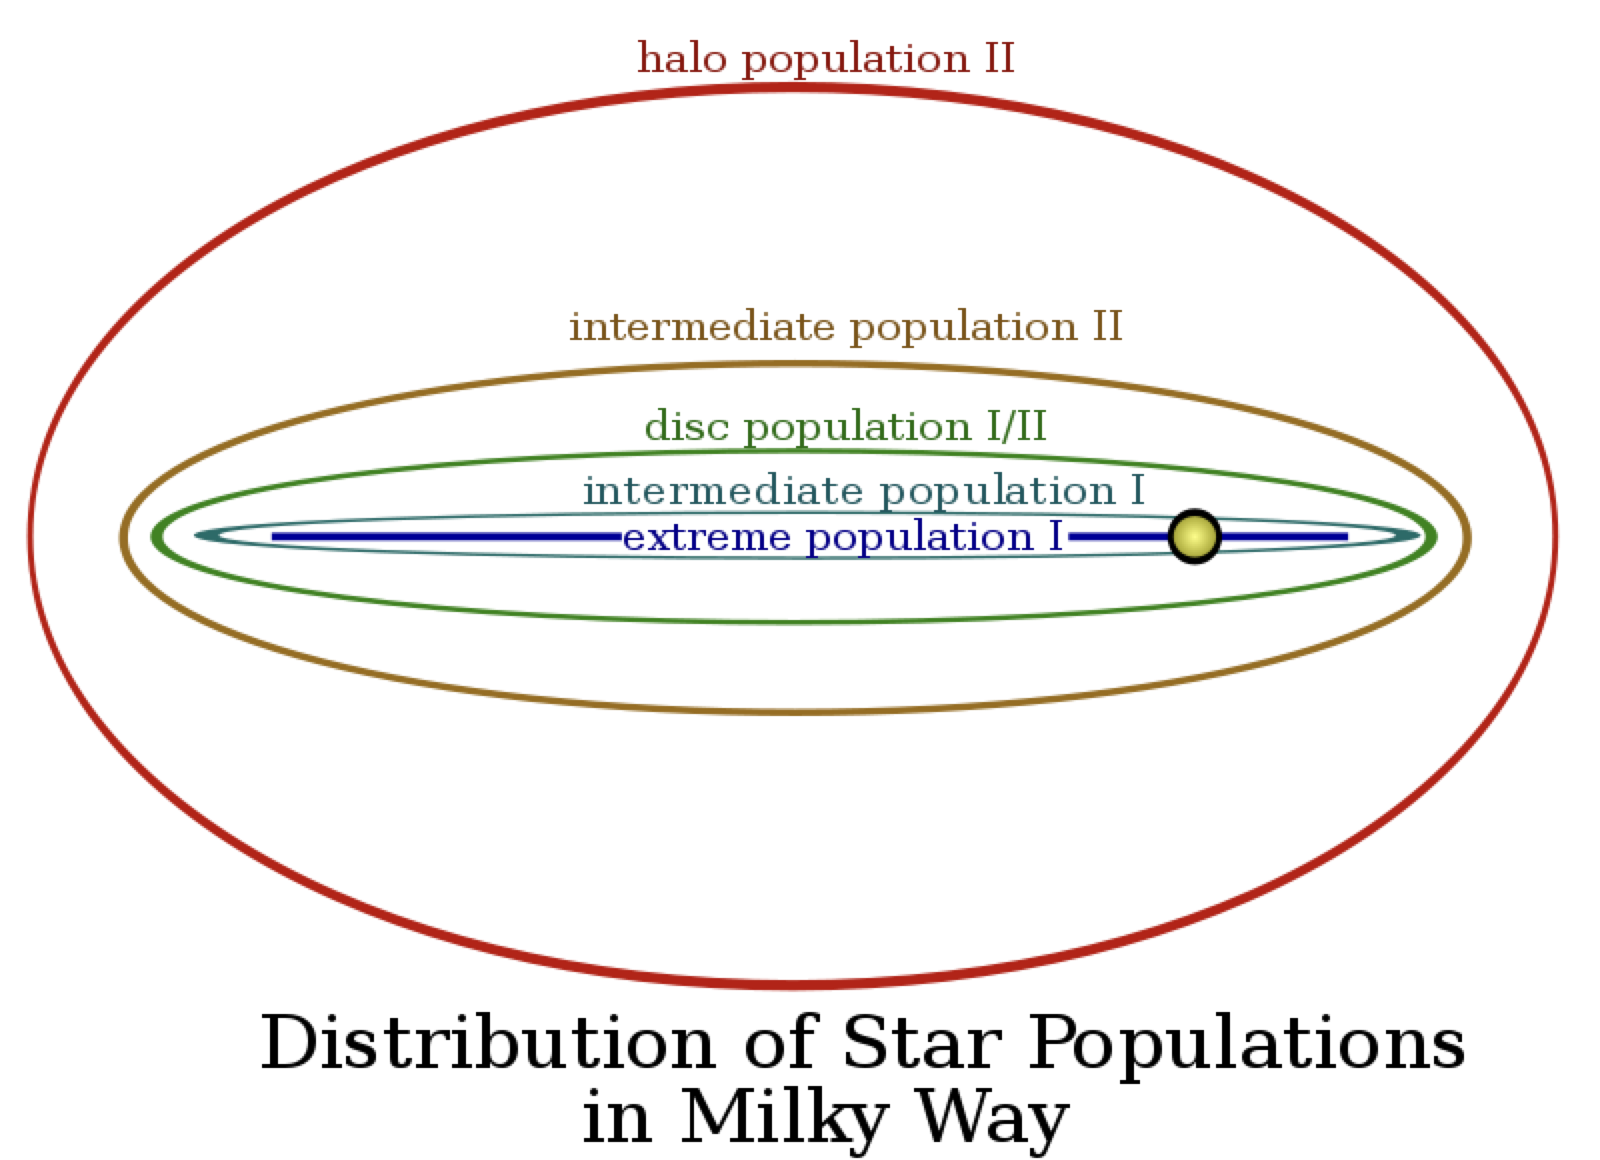
\includegraphics[scale=0.20]{ghz.png}

 \column{0.45\textwidth}
 
 REH suggests that much of the known universe, including large parts of our galaxy, are ``dead zones'' unable to support complex life. Those parts of a galaxy where complex life is possible make up the galactic habitable zone (GHZ), which is primarily characterized by distance from the Galactic Center (GC).
%The galactic habitable zone is the region of a galaxy in which life might most likely develop. The concept of a galactic habitable zone analyzes various factors, such as metallicity (the presence of elements heavier than hydrogen and helium) and the rate and density of major catastrophes such as supernovae, and uses these to calculate which regions of a galaxy are more likely to form terrestrial planets, initially develop simple life, and provide a suitable environment for this life to evolve and advance. In the case of the Milky Way, its galactic habitable zone is commonly believed to be an annulus with an outer radius of about 10 kiloparsecs (33,000 ly) and an inner radius close to the Galactic Center.
\end{columns}
\end{frame}

\begin{frame}
\begin{itemize}
\item As that distance to the GC increases, {\bf star metallicity} (the presence of elements heavier than hydrogen and helium) declines. Metals are necessary for the formation of terrestrial planets.
\item {\bf The X-ray and gamma ray radiation} from the black hole at the galactic center, and from nearby neutron stars, becomes less intense as distance increases. Thus the early universe, and present-day galactic regions where stellar density is high and supernovae are common, will be dead zones.
\item{\bf Gravitational perturbation} of planets and planetesimals by nearby stars becomes less likely as the density of stars decreases. Hence the further a planet lies from the GC or a spiral arm, the less likely it is to be struck by a large bolide which could extinguish all complex life on a planet.
\end{itemize}

\vspace{0.5cm}
\begin{block}{}
Item \#1 rules out the outermost reaches of a galaxy; \#2 and \#3 rule out galactic inner regions. Hence a galaxy's habitable zone may be a relatively narrow ring of adequate conditions sandwiched between its uninhabitable center and outer reaches. Lineweaver et al. calculate calculate the GHZ to be a ring 7 to 9 kiloparsecs in radius, including no more than 10\% of the stars in the Milky Way.
\end{block}
\end{frame}

\begin{frame}
\frametitle{Rare Milky Way}

\begin{itemize}
\item According to REH, our own galaxy is unusually quiet and dim (see below), representing just 7\% of its kind (even so, this would still represent more than 200 billion galaxies in the known universe).

\item Also, our galaxy also appears unusually favorable in suffering fewer collisions with other galaxies over the last 10 billion years, which can cause more supernovae and other disturbances. In addition, the Milky Way's central black hole seems to have neither too much nor too little activity.

\item A habitable planetary system must maintain its favorable location long enough for complex life to evolve. A star with an eccentric (elliptical or hyperbolic) galactic orbit will pass through some spiral arms, unfavorable regions of high star density; thus a life-bearing star must have a galactic orbit that is nearly circular, with a close synchronization between the orbital velocity of the star and of the spiral arms. The orbit of the Sun around the center of the Milky Way is indeed almost perfectly circular, with a period of 226 Myrs, closely matching the rotational period of the galaxy. 
%\item REH predicts that the Sun should rarely, if ever, have passed through a spiral arm since its formation. Masters has calculated that the orbit of the Sun takes it through a major spiral arm approximately every 100 million years.[13] Some researchers have suggested that several mass extinctions do indeed correspond with previous crossings of the spiral 

\end{itemize}
\end{frame}

\begin{frame}
\frametitle{Earth, the Solar System and the and Goldilocks effect}

\begin{columns}
\column{0.45\textwidth}

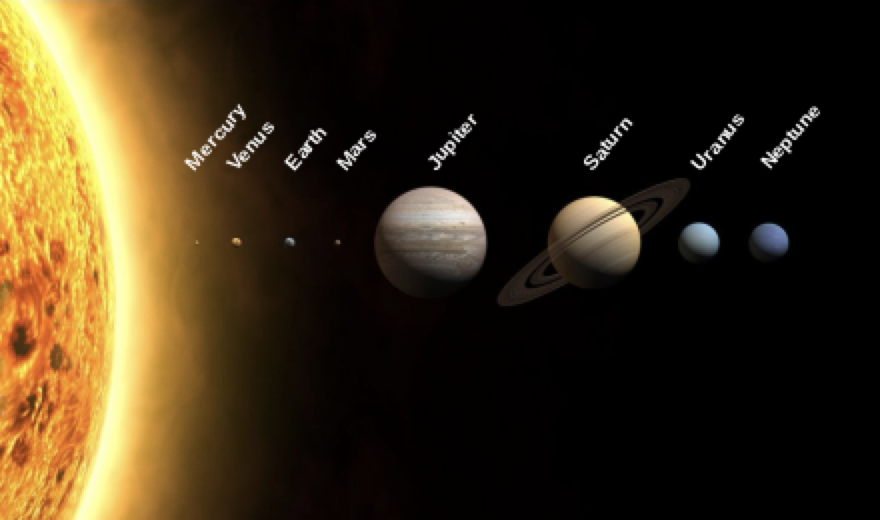
\includegraphics[scale=0.35]{solarsystem}

Observations of exoplanets have shown that arrangements of planets similar to the Solar System are rare. Most planetary systems have super-Earths, several times larger than Earth, close to their star, whereas the Solar System's inner region has only a few small rocky planets. Only 10\% of stars have giant planets similar to Jupiter and Saturn, and those few rarely have stable, nearly circular orbits distant from their star.
 \column{0.55\textwidth}

According to the REH, our planet has an improbable orbit in the very narrow habitable zone (dark green) around the Sun that makes possible:
\begin{itemize}
\item {\bf Liquid water}, necessary for complex life.
\item {\bf An atmosphere}, neither too thin (Mars), nor too thick (Venus), with the right amount of greenhouse effect (currently being disturbed by humans).
\item {\bf A planetary system} capable of sustaining complex life, with small, rocky inner planets and massive outer gas giants which act as ``celestial vacuum cleaners'' avoiding frequent catastrophic asteroid collisions in inner planets.
 

%Konstantin Batygin and colleagues argue that these features can be explained if, early in the history of the Solar System, Jupiter and Saturn drifted towards the Sun, sending showers of planetesimals towards the super-Earths which sent them spiralling into the Sun, and ferrying icy building blocks into the terrestrial region of the Solar System which provided the building blocks for the rocky planets. The two giant planets then drifted out again to their present positions. In the view of Batygin and his colleagues: "The concatenation of chance events required for this delicate choreography suggest that small, Earth-like rocky planets – and perhaps life itself – could be rare throughout the cosmos."[25] 
\end{itemize}


\end{columns}
\end{frame}

\begin{frame}
\frametitle{A planet of the right size}

\begin{columns}
\column{0.45\textwidth}

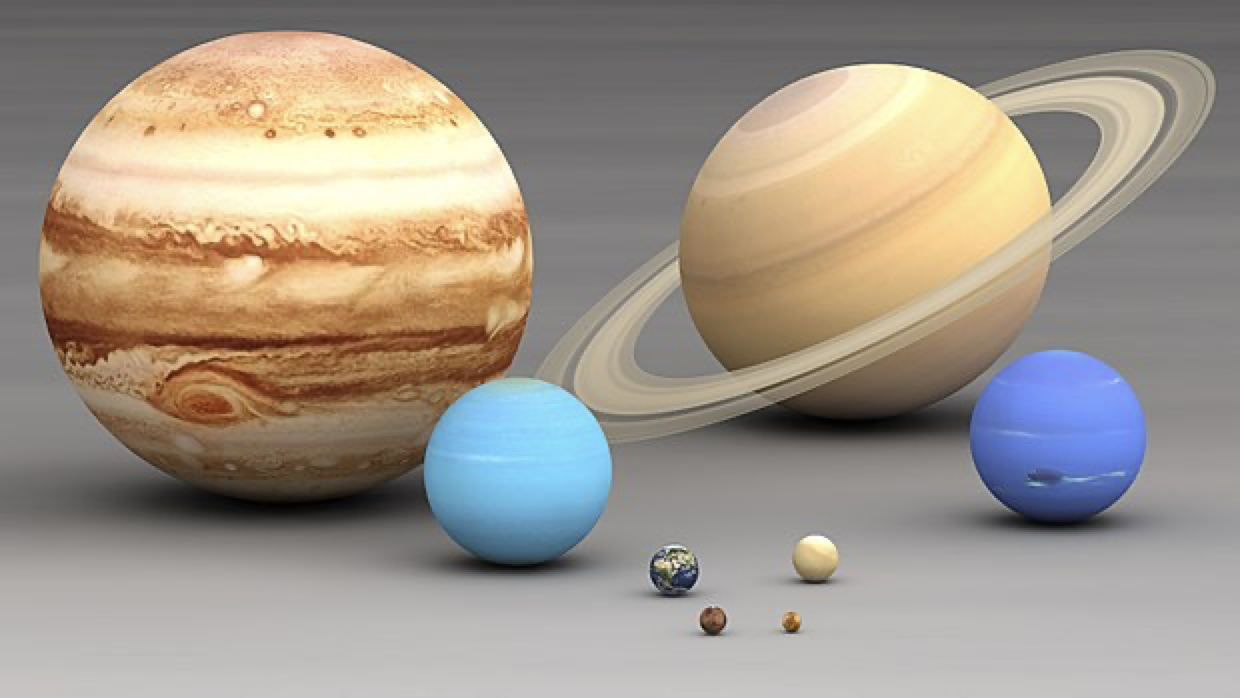
\includegraphics[scale=0.25]{planetsize}

Planets of the Solar System, shown to scale. Rare Earth argues that complex life cannot exist on large gaseous planets like Jupiter and Saturn (top row) or Uranus and Neptune (top middle) or smaller planets such as Mars and Mercury.

 \column{0.55\textwidth}
REH argues that life requires terrestrial planets like Earth. Gas giants lack a rocky surface (or a liquid ocean), making complex life unlikely. On the other hand,
a planet that is too small (Mars) cannot maintain much atmosphere, rendering its surface temperature low and variable and oceans impossible. A small planet will also tend to have a rough surface, with large mountains and deep canyons. The core will cool faster, and plate tectonics may be brief or entirely absent. A planet that is too large will retain too dense an atmosphere, like Venus. Although Venus is similar in size and mass to Earth, its surface atmospheric pressure is 92 times that of Earth, and its surface temperature is 735 K (462 °C; 863 °F). The early Earth once had a similar atmosphere, but may have lost it in the giant impact event which formed the Moon.

\end{columns}
\end{frame}

\begin{frame}
\frametitle{Plate tectonics and biodiversity}

\begin{columns}
\column{0.45\textwidth}

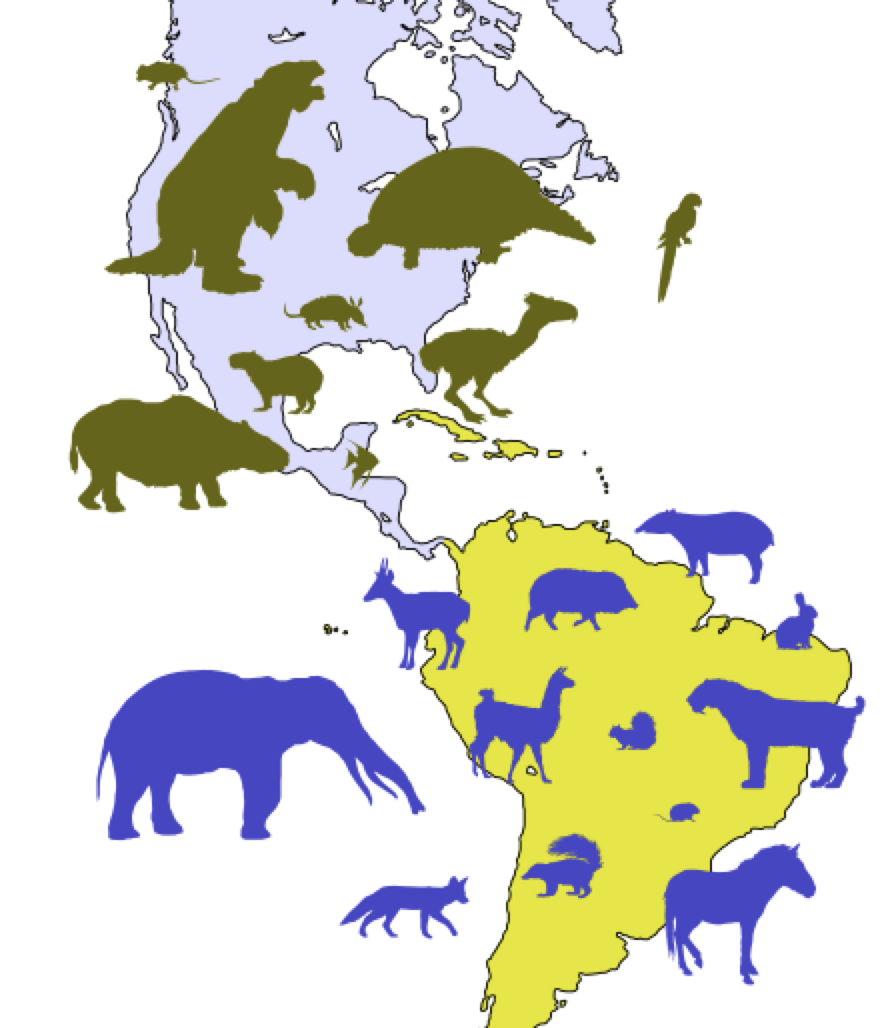
\includegraphics[scale=0.25]{tectonics}

Plate tectonics and as a result continental drift and the creation of separate landmasses would create diversified ecosystems and biodiversity, one of the strongest defences against extinction. 

 \column{0.55\textwidth}
An example of species diversification and later competition on Earth's continents is the Great American Interchange. North and Middle America drifted into South America at around 3.5 to 3 Ma. The fauna of South America had already evolved separately for about 30 million years, since Antarctica separated, but after the merger many species were wiped out, mainly in South America, by competing North American animals.

\end{columns}
\end{frame}

\begin{frame}
\frametitle{A large (and unlikely) Moon}

\begin{columns}
\column{0.45\textwidth}

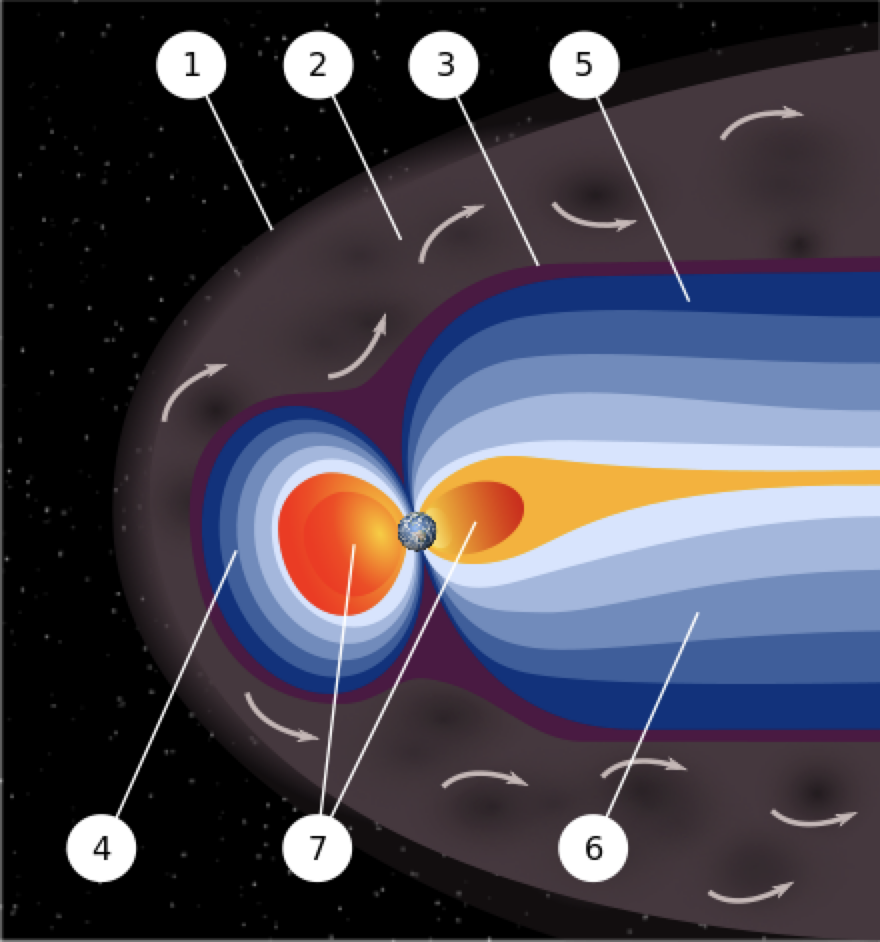
\includegraphics[scale=0.25]{magnetosphere}

The Moon may be essential to maintaining our planet's magnetic shield by continually acting upon the metallic core as dynamo, thus protecting the surface of Earth from charged particles and cosmic rays, and helping to ensure the atmosphere is not stripped over time by solar winds.

 \column{0.55\textwidth}
The Moon could have been formed from the impact of a Mars-sized body (Theia), with the young Earth. This giant impact also gave the Earth its axial tilt (inclination) and velocity of rotation. Rapid rotation reduces the daily variation in temperature and makes photosynthesis viable. The impact may also have initiated plate tectonics, without which the continental crust would cover the entire planet, leaving no room for oceanic crust.

If the Earth had no Moon, the ocean tides resulting solely from the Sun's gravity would be only half that of the lunar tides. A large satellite gives rise to tidal pools, which may be essential for the formation of complex life.
It also increases the likelihood of plate tectonics through the effect of tidal forces on the planet's crust.
\end{columns}
\end{frame}

\begin{frame}
\frametitle{A Rare Atmosphere}

\begin{columns}
\column{0.45\textwidth}

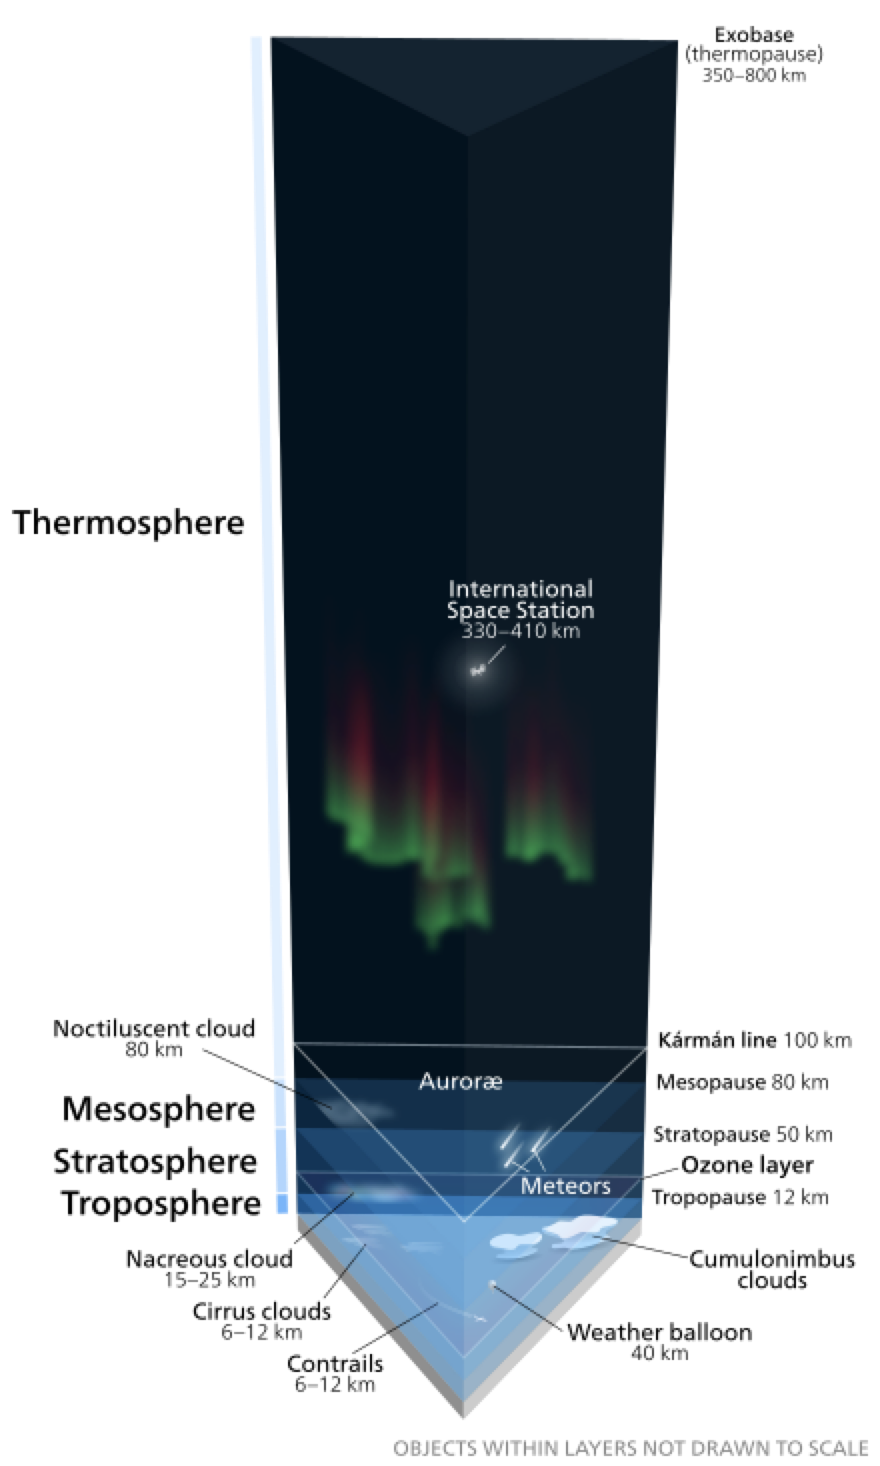
\includegraphics[scale=0.25]{atmosphere}


 \column{0.55\textwidth}
A terrestrial planet must be the right size, like Earth and Venus, in order to retain an atmosphere (but in the case of Venus the atmosphere is too dense). On Earth, once the giant impact of Theia thinned Earth's atmosphere, other events were needed to make the atmosphere capable of sustaining life. {\bf The Late Heavy Bombardment} reseeded Earth with water lost after the impact. The development of an {\bf ozone layer} generated a protective shield against ultraviolet (UV) sunlight. {\em Nitrogen and carbon dioxide} are needed in a correct ratio for life to form. {\bf Lightning} is needed for nitrogen fixation.  {\bf Precipitation} is needed to have a stable water cycle. A proper atmosphere must reduce {\bf diurnal temperature variation}.
\end{columns}
\end{frame}


\begin{frame}
\frametitle{Rare Complex Life}

\begin{columns}
\column{0.45\textwidth}

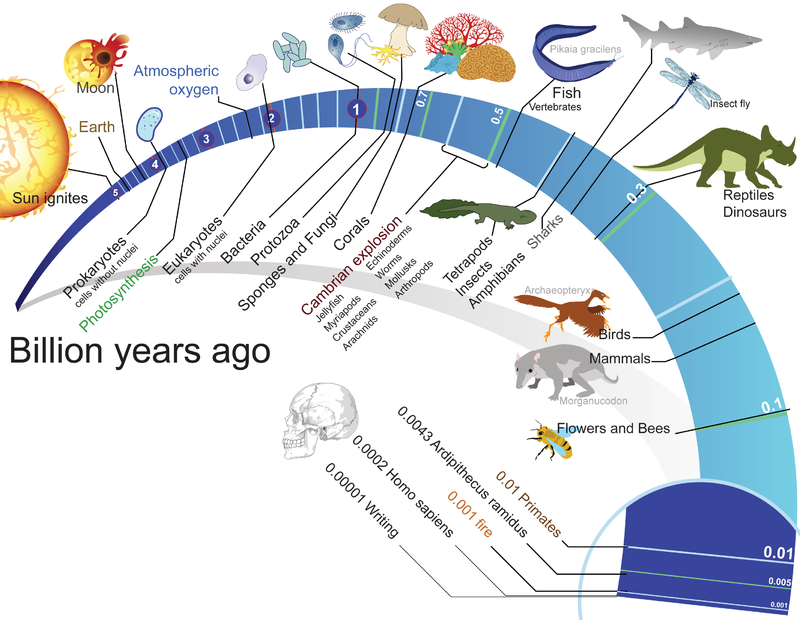
\includegraphics[scale=0.40]{evolutionlife}


 \column{0.55\textwidth}
Prokaryotes appeared $\sim$ 4 Gyr ago, early after the collision with Theia. Eukariotes only appeared 2 Gyr ago, and the Cambrian explosion 0.5 GYr ago.  
All eukariotes share a common ancestor, which implies that this event can only have happened once. Lane and others argue that prokaryotes lack the cellular architecture to evolve into eukaryotes because a bacterium expanded up to eukaryotic proportions would have tens of thousands of times less energy available to power its metabolism. Two billion years ago, one simple cell incorporated itself into another, multiplied, and evolved into mitochondria that supplied the vast increase in available energy that enabled the evolution of complex eukaryotic life. If this incorporation occurred only once in four billion years or is otherwise unlikely, then life on most planets remains simple.


\end{columns}
\end{frame}

\begin{frame}
\frametitle{Rare Good Luck}
\begin{itemize}
\item Civilizations on Earth have existed for about 12,000 years, and radio communication reaching space has existed for little more than 100 years. Relative to the age of the Solar System ($\sim$4.57 Ga) this is a short time, in which extreme climatic variations, super volcanoes, and large meteorite impacts were absent. These events would severely harm intelligent life, as well as life in general.
\item For example, the Permian-Triassic mass extinction, caused by widespread and continuous volcanic eruptions in an area the size of Western Europe, led to the extinction of 95\% of known species around 251.2 Ma ago. About 65 million years ago, the Chicxulub impact at the Cretaceous--Paleogene boundary ($\sim$65.5 Ma) on the Yucatán peninsula in Mexico led to a mass extinction of the most advanced species at that time (while at the same time facilitated the expansion of the mammals)
\end{itemize}
\end{frame}


\begin{frame}
\frametitle{Rare Intelligence}
\begin{itemize}
\item REH also argues that the evolutionary path from primitive Cambrian chordates to Homo sapiens, was a highly improbable event. For example, the large brains of humans have marked adaptive disadvantages, requiring as they do an expensive metabolism, a long gestation period, and a childhood lasting more than 25\% of the average total life span.
\item The fact that humans did not already go extinct may on itself be ``rare''.

https://www.nature.com/articles/d41586-023-02712-4

\item In many aspects, humans are extremely ``unlikely'': bipedalism, eye-hand coordination
(whichvpermits dextrous manipulations of the physical environment with the hands) and a vocal apparatus enabling speech which in turn makes possible for humans to interact cooperatively, to share knowledge, and to acquire a culture.
The capability of formulating abstractions to a degree permitting the invention of mathematics, and the discovery of science and technology may also be very rare and unique of Sapiens (e.g, not sufficiently developed in our close cousins, the Neanderthals). Last but not least, humans have acquirer their current scientific and technological sophistication only very recently.
\end{itemize}
\end{frame}

\begin{frame}
\frametitle{Criticism to REH}

\begin{columns}
\column{0.45\textwidth}

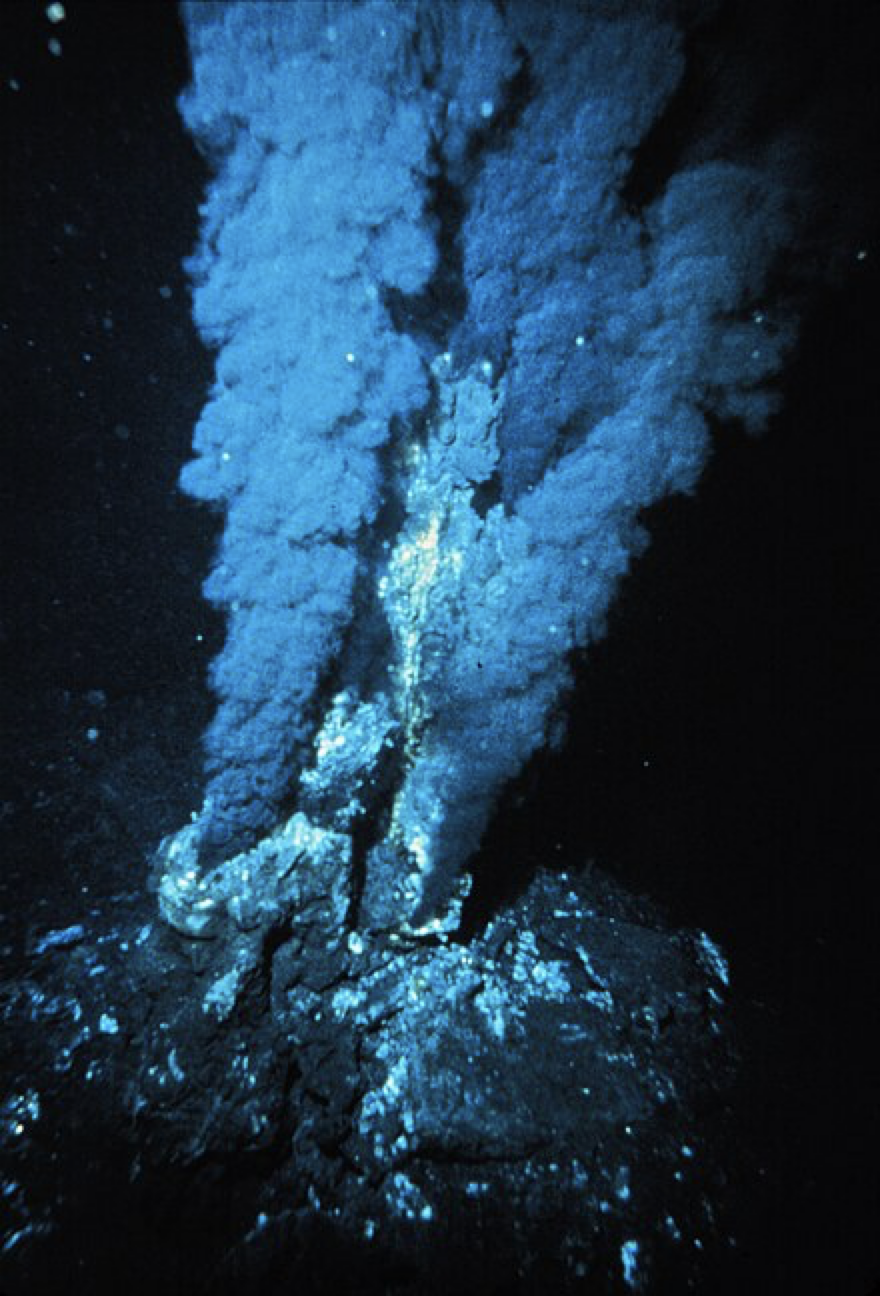
\includegraphics[scale=0.30]{geiser}

Complex life may exist in environments similar to black smokers on Earth.
 \column{0.55\textwidth}


REH could be an example of circular reasoning, which simply describes how life (and intelligence) arose on Earth. The improbable sequence of events leading to complex life and intelligence on Earth could have been mirrored by other sequence of improbable events elsewhere.  

Almost all assertions of REH have been challenged. A few examples: Exoplanets around main sequence stars are being discovered in large numbers; Rocky planets orbiting within habitable zones may not be rare; The requirement for a system to have a Jovian planet as protector has been challenged (Kastings, 2001, Horner and Jones, 2008). Plate tectonics may not be unique to Earth or a requirement for complex life; Free oxygen may be neither rare nor a prerequisite for multicellular life; A magnetosphere may not be rare or a requirement.
\end{columns}
\end{frame}

\begin{frame}
\frametitle{The example of exoplanets}

\begin{columns}
\column{0.45\textwidth}

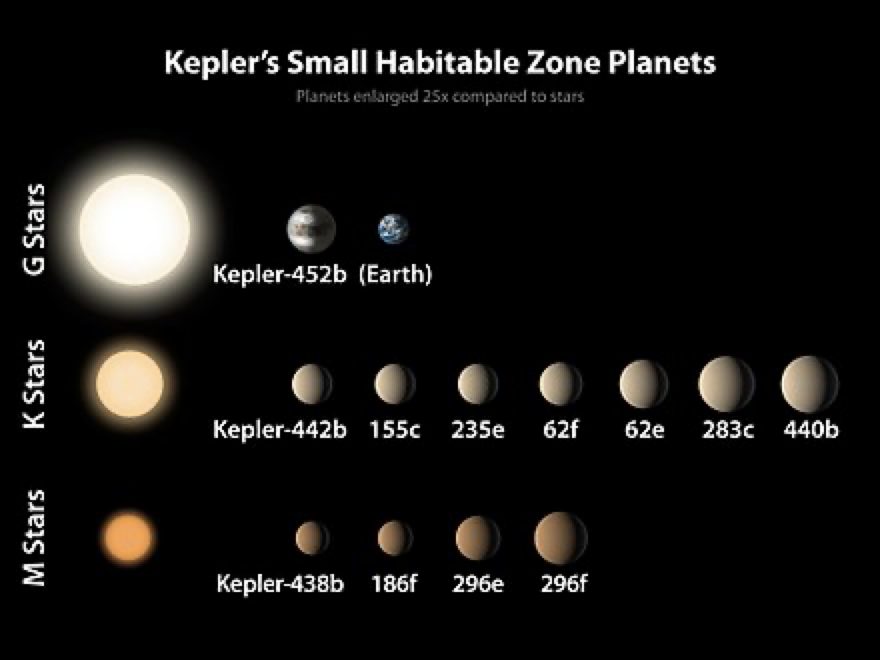
\includegraphics[scale=0.30]{exoplanets}

Planets similar to Earth in size are being found in relatively large number in the habitable zones of similar stars. 
 \column{0.55\textwidth}
 
 An increasing number of extrasolar planet discoveries are being made, with 5,506 planets in 4,065 planetary systems. Though planets the size of Earth are difficult to detect and classify, scientists now think that rocky planets are common around Sun-like stars. Astronomers using the Kepler space telescope's data have estimated that about one-fifth of G-type and K-type stars (sun-like stars and orange dwarfs) are expected to have an Earth-sized or super-Earth-sized planet (1--2 Earths wide) close to an Earth-like orbit yielding about 8.8 billion of them for the entire Milky Way.

%Current technology limits the testing of important Rare Earth criteria: surface water, tectonic plates, a large moon and biosignatures are currently undetectable. Though planets the size of Earth are difficult to detect and classify, scientists now think that rocky planets are common around Sun-like stars.[75] The Earth Similarity Index (ESI) of mass, radius and temperature provides a means of measurement, but falls short of the full Rare Earth criteria.[
 \end{columns}
\end{frame}

